\documentclass[11pt,letterpaper]{article}
\usepackage[margin=1.05in,includeheadfoot]{geometry}
\usepackage[T1]{fontenc}
\usepackage[utf8]{inputenc}
\usepackage{lmodern}
\usepackage{amsmath,amssymb,amsthm,mathtools,microtype}
\usepackage{booktabs,tabularx,array,enumitem,tikz}
\usepackage{hyperref}
\hypersetup{colorlinks=true,linkcolor=black,citecolor=black,urlcolor=blue,
  pdftitle={Simultaneous Embedding with Fixed Edges for Two Graphs},
  pdfauthor={}}
\usepackage{fancyhdr}
\setlength{\headheight}{13.6pt}
\pagestyle{fancy}
\fancyhf{}
\fancyhead[L]{\small\itshape Simultaneous Embedding with Fixed Edges}
\fancyhead[R]{\small\thepage}
\renewcommand{\headrulewidth}{0pt}
\setlength{\parindent}{1.3em}
\setlength{\parskip}{0pt}
\setlist{topsep=3pt,itemsep=1pt,parsep=1pt}
\allowdisplaybreaks[2]
\newtheorem{theorem}{Theorem}[section]
\newtheorem{lemma}[theorem]{Lemma}
\newtheorem{proposition}[theorem]{Proposition}
\newtheorem{corollary}[theorem]{Corollary}
\theoremstyle{definition}
\newtheorem{definition}[theorem]{Definition}
\newtheorem{remark}[theorem]{Remark}
\newcommand{\Ftwo}{\mathbb F_2}
\newcommand{\cc}{\operatorname{cc}}
\newcommand{\rev}{\operatorname{rev}}
\newcommand{\side}{\operatorname{side}}
\newcommand{\gap}{\operatorname{gap}}
\newcommand{\orcyc}{\operatorname{or}}
\newcommand{\SEFE}{\ensuremath{\mathrm{SEFE\text{-}2}}}
\newcommand{\SP}{\ensuremath{\mathrm{SP}}}
\title{Simultaneous Embedding with Fixed Edges\\[3pt]for Two Graphs}
\author{}
\date{Draft --- November 2026}
\begin{document}
\maketitle
\vspace{-1.4em}
\begin{abstract}
We describe a deterministic polynomial-time algorithm for simultaneous
embedding with fixed edges of two planar graphs, without restrictions on
the common graph, and give a procedure constructing compatible
combinatorial embeddings.  The central intermediate result characterizes
when prescribed embeddings of the colour blocks can be assembled: a
common order of the shared darts must respect both block partitions,
and every component outside a common block must have a face incident
with all its attachments and consistent with its prescribed colour lobes.

To choose the block embeddings, we retain complete face sectors at common
P-nodes.  A component attached exactly at the two poles may occupy any
of several sectors, while an additional attachment restricts each
potentially nonaffine side observation to at most two possibilities.
This yields a constrained-planarity language with partial bijections
between finite domains and affine equations on Boolean variables.  We
extend the Synchronized Planarity reductions to this language and give
forward and inverse witness transformations for every operation.
A conservative bound for the resulting algorithm is
$O((N+1)^{60})$, where $N$ is the total input size.
\end{abstract}
\section{Introduction}
\label{sec:introduction}

Let $G_1=(V,E_1)$ and $G_2=(V,E_2)$ be planar graphs.  A
\emph{simultaneous embedding with fixed edges} (\SEFE) is a pair of planar
drawings that represent every vertex by the same point and every edge of
$H=(V,E_1\cap E_2)$ by the same curve.  Edges belonging exclusively to
different input graphs may cross.  The distinction from drawing the union
$G_1\cup G_2$ planarly is essential: the union need not be planar.

For three or more input graphs the problem is
NP-complete~\cite{gjpss06}.  For two input graphs its complexity has
remained open; it is stated as an open problem in recent
work~\cite{fpr,isaac,ramsey}.  The general decision problem has resisted the
usual planarity-decomposition techniques.  The connected-common-graph case
was first solved in polynomial time by Fulek and T\'oth~\cite{atomic}, and
in quadratic time by Synchronized Planarity~\cite[Theorem~16]{bfr}, but
disconnected common graphs carry information not determined by local
rotations.  Even when the two
colours agree on the rotation of every common edge, a component of $H$ may
occupy different faces of another common component.  These relative
positions interact at common cutvertices and at separation pairs of the
input graphs~\cite{brdisconnect,bkr}.

\begin{theorem}\label{thm:main}
There is a deterministic polynomial-time algorithm which, given two planar
graphs $G_1,G_2$ on the same vertex set, decides whether they admit a
simultaneous embedding with fixed edges.  On a positive instance it
constructs compatible combinatorial embeddings, including the relative
positions of all connected components of their common graph.  No
connectivity, degree, or block restriction is imposed on the common graph.
\end{theorem}

The proof is constructive.  With
\[
 N=|V|+|E_1|+|E_2|,
\]
a deliberately generous bound for the algorithm presented here is
$O((N+1)^{60})$.  We make no attempt to optimize this exponent.

\paragraph{Face compatibility.}
The first step separates the choice of block embeddings from their
assembly.  Suppose an oriented planar embedding has already been selected
for every biconnected block of each input graph.  Compatible orders of the
common darts at a vertex are necessary, but not by themselves sufficient.
For each common block $K$ and each component $Z$ of
$(G_1\cup G_2)-V(K)$, all of $Z$ must occupy one face of $K$.  That face
must be incident with every attachment of $Z$ and must agree with the
positions of the pieces of $Z$ already prescribed within the colour
blocks containing $K$.

We prove that these requirements are also sufficient
(Theorem~\ref{rep:thm:repair}).  The local repair is described by a tree
whose nodes represent common blocks and the regions between them.  Its
contour constructs compatible orders without changing any prescribed
colour-block embedding.  The theorem applies to disconnected $H$, to
isolated common vertices, and to arbitrarily many common blocks meeting
at a cutvertex.

\paragraph{Face sectors rather than individual side bits.}
The second step is to choose the colour-block embeddings subject to the
face requirements.  After the separation-pair preprocessing of
Bl\"asius--Karrer--Rutter~\cite[Lemmas~2--4 and Theorem~2]{bkr}, every
P-node of a common block has a known cyclic order up to reversal
(Section~\ref{gen:porders} treats a real common pole edge); see also
Fink--Pfretzschner--Rutter~\cite[Lemma~4(c)]{fpr}.  A binary order choice,
however, does not remove the many possible faces between the expansions
of a P-node.

Let a common P-node have poles $p,q$ and reference directions
$e_0,\ldots,e_{k-1}$.  Its faces incident with both poles correspond to
the $k$ sectors between successive directions.  We retain a sector as one
variable with $k$ possible values instead of asking separately on which
side of several common cycles a component lies.  This is essential:
orientations of several triples at one freely permutable P-node need not
form an affine Boolean relation.

The crucial structural distinction is determined by the attachment set
$A_K(Z)=N_{G_1\cup G_2}(Z)\cap V(K)$.
\begin{itemize}[leftmargin=1.4em]
\item If $A_K(Z)=\{p,q\}$ for the poles of a common P-node, we keep the
      \emph{entire face name} of $Z$, and compare it directly with the face
      names of the relevant colour lobes.
\item Otherwise a new vertex adjacent to all of $A_K(Z)$ witnesses an
      eligible face of $K$.  We compare that face with the faces of the
      colour lobes using a fixed cycle basis of $K$.
\end{itemize}
\begin{figure}[t]
\centering
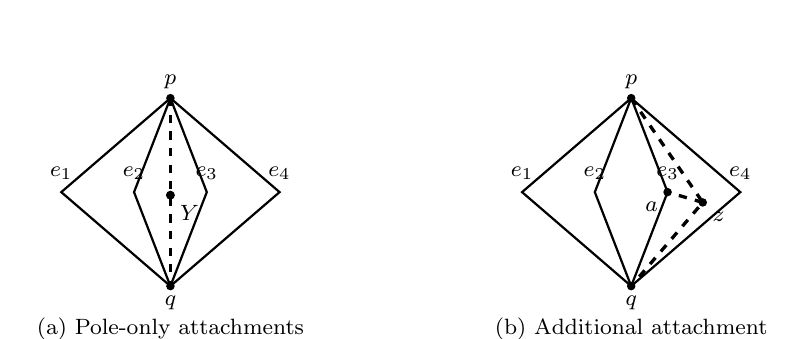
\begin{tikzpicture}[scale=.77, every node/.style={font=\footnotesize}]
  \begin{scope}[xshift=-3.8cm]
    \coordinate (p) at (0,1.55); \coordinate (q) at (0,-1.55);
    \foreach \x/\lab in {-1.8/1,-.6/2,.6/3,1.8/4} {
      \draw[thick] (p) -- (\x,0) -- (q);
      \node[above=1pt] at (\x,0) {$e_{\lab}$};
    }
    \fill (p) circle(2pt) node[above] {$p$};
    \fill (q) circle(2pt) node[below] {$q$};
    \coordinate (y) at (0,-.05);
    \draw[very thick, dashed] (p) -- (y) -- (q);
    \fill (y) circle(2.1pt) node[below right] {$Y$};
    \node at (0,-2.25) {(a) Pole-only attachments};
  \end{scope}
  \begin{scope}[xshift=3.8cm]
    \coordinate (p) at (0,1.55); \coordinate (q) at (0,-1.55);
    \foreach \x/\lab in {-1.8/1,-.6/2,.6/3,1.8/4} {
      \draw[thick] (p) -- (\x,0) -- (q);
      \node[above=1pt] at (\x,0) {$e_{\lab}$};
    }
    \coordinate (z) at (1.18,-.17);
    \draw[very thick, dashed] (p) -- (z) -- (q);
    \draw[very thick, dashed] (z) -- (.6,0);
    \fill (.6,0) circle(2pt) node[below left] {$a$};
    \fill (z) circle(2pt) node[below right] {$z$};
    \fill (p) circle(2pt) node[above] {$p$};
    \fill (q) circle(2pt) node[below] {$q$};
    \node at (0,-2.25) {(b) Additional attachment};
  \end{scope}
\end{tikzpicture}
\caption{Schematic face choices around a common P-node.  A component
attached only at $p,q$ may use any sector.  With an additional
attachment in the expansion $e_3$, its face must border that expansion.
Dashed edges denote private or auxiliary attachments; the drawing
shows one permissible placement in each case.}
\label{fig:sector-dichotomy}
\end{figure}

The only potentially nonaffine side observation in the second case comes
from an entire colour lobe attached at a common P-pair.  Since $Z$ has an
additional attachment, at most two sectors can contain it.  On this
restricted domain every side observation is a Boolean affine function.
Importantly, this restriction is applied \emph{in addition to}, not in
place of, the original face comparisons.

\paragraph{An exact constraint language.}
The resulting problem is a restricted extension of the Synchronized
Planarity problem of Bl\"asius--Fink--Rutter~\cite{bfr}.  A marked
P-vertex has one reference order of its marked darts, up to reversal, and
an unmarked dart may be assigned to a named sector.  Finite-domain
variables are related only by unary restrictions and partial bijections;
designated Boolean variables may also satisfy affine equations over
$\Ftwo$.  This language is tractable because a connected component of
partial-bijection constraints has at most two assignments as soon as it
contains a Boolean variable.  The residual Boolean system is solved by
Gaussian elimination.

The graph-theoretic work is to show that the ordinary Synchronized
Planarity reduction operations preserve these extra observations, in
\emph{both} witness directions.  We do this for encapsulation, joining,
propagation, the reordering of parallel expansions, self-pipes, and the
pipe-free terminal instance.  Two recurring tools are the injective
transport of a corner of a marked embedding subtree to a frontier sector
and the preservation of complete sector categories when whole expansion
intervals are reordered.  The case of two marked darts requires an
independent frame bit, even though their cyclic order is vacuous.

The three principal results are an assembly theorem
(Theorem~\ref{rep:thm:repair}), an exact compilation
(Theorem~\ref{gen:compilation}), and a solver for the complete-sector
constraint language (Theorem~\ref{cse:main}).  Their composition proves
Theorem~\ref{thm:main}.

\paragraph{Related work and scope.}
The preprocessing and the role of relative positions in disconnected
common graphs originate in~\cite{brdisconnect,bkr}.  Synchronized
Planarity gives a polynomial-time framework for several constrained
embedding problems~\cite{bfr}.  General Simultaneous PQ-Ordering is not
used as an algorithmic oracle: only its restricted variants are known to
be efficiently solvable~\cite{pqordering}.  Nor do we invoke Schaefer's
conjectured strong Hanani--Tutte theorem for
\SEFE{}~\cite[Conjecture~6.20]{schaefer}.  That conjecture is false:
Gutwenger, Mutzel and Schaefer~\cite{gms2014} turned the clustered-planarity
counterexamples of Fulek, Kyn\v{c}l, Malinovi\'c and P\'alv\"olgyi into
counterexamples to it (see~\cite[p.~6]{fkmp2015}
and~\cite[p.~137]{fps2017}).  The closest precedent for our engine is
Pfretzschner's extension of Synchronized Planarity by equations between
triple orientations, which solves \SEFE{} when both input graphs are
biconnected and have maximum degree four~\cite[Chapter~8]{pfretzschner};
the present language instead retains complete sector categories.
Carmesin and Turner~\cite{temporal} give a polynomial-time algorithm for
2-connected temporal sequences, and state that their framework also
resolves a rooted-tree variant of \SEFE{}.
A cycle-based repair construction for cactus
common graphs was developed in the preliminary manuscript~\cite{cactus};
we treat the results needed here directly, rather than importing that
manuscript as a theorem.

\paragraph{Organization.}
Section~\ref{sec:normalization} fixes conventions and proves the
normalization steps used subsequently.
Section~\ref{rep:section} proves the face-list assembly criterion.
Section~\ref{gen:section} constructs the constraint instance from an
arbitrary normalized SEFE instance.
Section~\ref{cse:section} gives the complete-sector solver, including the
inverse transformations.
Section~\ref{sec:composition} finishes the algorithm and its size bound.
Counterexamples to tempting weaker conditions and the finite checks are
separated into Appendix~\ref{sec:verification}.

\section{Preliminaries and normalization}
\label{sec:normalization}

The constructions below operate on finite, simple, undirected input graphs.
This entails no restriction on the theorem if the input convention permits
loops or parallel edge identities. Replace each input edge by a path of
length three with two fresh internal vertices. For a common edge use the
same path in both colours; for a private edge give the new vertices
isolated copies in the other colour. The resulting graphs are simple and
have total size $O(N)$. A SEFE extends by choosing subdivision points away
from all other drawing features. Conversely, suppress the path's internal
vertices in its colour or colours and delete their isolated copies in the
other colour. This restores the original edge curves and is an exact
linear-size reduction. Empty graphs and union components with at most two
vertices after this step are handled directly.

Auxiliary SPQR skeletons and Synchronized Planarity instances may be loopless
multigraphs; a digon is then a simple cycle. Drawings are considered on an
oriented sphere. Selecting a point outside the finite drawing converts the
result to the plane. A block is a maximal biconnected subgraph or a bridge.
An isolated vertex belongs to no edge block.

A rotation system specifies a cyclic order of incident darts at every
vertex. It is planar if each connected component has Euler characteristic
$|V|-|E|+f=2$, where faces are obtained by tracing the dart successor
permutation, with $f=1$ for an isolated-vertex component. For a connected graph this determines its oriented spherical
embedding. For a disconnected graph one must additionally record the face
of each component containing every other component. These data can be
represented by a component--region containment tree. Equal rotations alone
are therefore insufficient in the disconnected case.

We use the common-embedding criterion: a pair has a SEFE exactly when
planar embeddings of its two colours induce the same embedding of $H$,
including relative component positions \cite[Theorem~4]{junger}. To see the sufficiency,
identify orientation-preserving regular neighbourhoods of corresponding
embedded common components. Their matching face positions identify the
remaining complementary regions. Extend the boundary identifications
through these planar regions to an orientation-preserving homeomorphism.
Applying it to one colour identifies the whole common drawing. Isolated
common vertices are matched as marked points in the corresponding regions.
The standard topological facts behind this sketch are stated at the end of
Section~\ref{rep:global}.

For a cyclic order $\sigma$ and distinct elements $a,d,b$, put
\[
 \orcyc_\sigma(a,d,b)=
 \begin{cases}0,&d\text{ occurs between }a\text{ and }b\text{ going forward},\\
 1,&\text{otherwise}.
 \end{cases}
\]
Reflection complements this bit. A directed cycle $C$ has left side $0$
and right side $1$. With outgoing and incoming darts $c_{\rm out},c_{\rm in}$
at $v$, the local gap of a noncycle dart $d$ is
$\gap(C,v,d)=\orcyc_{\rho_v}(c_{\rm out},d,c_{\rm in})$.
The connected component entered by $d$ after deleting $C$ is on that side.
For three leaves in a plane tree, their frontier orientation equals the
orientation of their three directions at their median. This follows by
reading the three disjoint contour excursions from the median.

\subsection{The published infrastructure used}

We use the classical block-cut and SPQR decompositions and their exact
embedding parameterization: R-skeleton reflections and P-skeleton cyclic
orders, opposite at their two poles, determine all block embeddings.
Substitution along twin virtual edges is the constructive inverse. We also
use ordinary deterministic planarity testing. These established algorithms
are sufficient at any polynomial running time; their linear bounds are
used only to simplify the estimates.

The other imported infrastructure is the ordinary Synchronized Planarity
algorithm of Bl\"asius--Fink--Rutter (BFR) \cite{bfr}: its graph operations,
their legal applicability, its reduction schedule and potential decrease.
Section~\ref{cse:section} proves the additional marking and observer
invariants, forward and backward, rather than assuming that the ordinary
algorithm preserves those extra constraints. The ordinary target has
Q-cells synchronizing fixed rotations up to reflection, and pipes requiring
full reversed correspondences between P-vertex rotations. The pipes form
a matching. No unrestricted simultaneous-ordering oracle is used.

\subsection{Connecting the colours without changing old common blocks}

First solve the connected components of $U=G_1\cup G_2$ independently.
Their solutions can occupy disjoint disks, so this is an equivalence in
both directions. In a connected union, if colour $i$ is disconnected,
some private edge $v_1v_2$ of the other colour joins distinct components
of $G_i$. The following fact is the connectivity normalization of
Bl\"asius--Rutter \cite[Section~2, Lemma~1 and Theorem~1]{brdisconnect}; we
give the nesting argument because it matters for arbitrary disconnected $H$.

\begin{lemma}[Cofacial relocation]
\label{norm:cofacial}
If an instance has a SEFE and an opposite-colour private edge $v_1v_2$
joins different components of $G_i$, it has a SEFE in which $v_1,v_2$
are incident with a common face of $G_i$.
\end{lemma}
\begin{proof}
In a SEFE the interior of the other-colour edge is in one face $f$ of
$H$. Near its endpoints it lies in faces $g_1,g_2$ of $G_i$, both
contained in $f$. If $g_1=g_2$, nothing is required. Otherwise let $Q_j$
be the colour-$i$ component containing $v_j$, and let $b$ be the face of
$Q_2$ containing $Q_1$. Let $\mathcal Y$ consist of $Q_2$ and all
colour-$i$ components lying in the complement of $b$.

Choose a small closed disk $\Delta'$ in $g_2$ near $v_2$, and a small
closed disk $\Delta$ in $g_1$ near $v_1$. Choose an orientation-preserving
sphere homeomorphism taking the complement of the interior of $\Delta'$
onto $\Delta$. Apply it to exactly the components in $\mathcal Y$.
They all fit in the empty disk $\Delta$, while all other colour-$i$
components remain outside. This is a planar drawing with the same
component rotations. The region outside $\Delta$ in $g_1$ and the image
of $g_2\setminus\operatorname{int}\Delta'$ join across $\partial\Delta$;
hence $v_1$ and the moved $v_2$ are cofacial.

It remains to verify the common embedding. Consider common components
$X$ outside $\mathcal Y$ and $X'$ inside. Before the move,
the complement of $b$, together with a small neighbourhood at $v_2$,
is connected, avoids $X$, contains $X'$, and meets the private edge
in $f$. Thus $X'$ is in the face of $X$ containing $f$. Afterwards it
lies in $\Delta\subset f$, so this position is unchanged.
Conversely, either $b$ itself, if $X'\subseteq Q_2$, or
$b\cup\Gamma_i(Q_2)$ otherwise, connects $X$ to $g_1$ while avoiding
$X'$. Its position relative to $X'$ is consequently the face containing
$f$. After the move, all unchanged components lie in the image of
$\operatorname{int}\Delta'$, the same transported face. Pairs both inside
or both outside retain their positions. The common rotations also
remain unchanged. The common-embedding criterion completes the SEFE.
\end{proof}

Add a fresh vertex $z$, a common edge $v_1z$, and a private colour-$i$
edge $zv_2$. This is an exact augmentation. For the forward direction use
Lemma~\ref{norm:cofacial}, put $z$ near $v_1$ in the shared local sector,
draw the small common segment $v_1z$ there, and complete the colour-$i$
arc to $v_2$ in its cofacial region. The other colour only receives the
small pendant common segment, adjacent to its existing edge $v_1v_2$.
For the local-sector claim, choose a disk at $v_1$ disjoint from the moved
components and from the relocation disk $\Delta$. The common drawing is
unchanged there. The common-embedding homeomorphism can be chosen to be
the identity on this disk: extend its complementary-region boundary maps
relative to the additional fixed disk. Thus the old opposite-colour edge
germ and its colour-$i$ sector $g_1$ are unchanged, and the two local
sectors used for the new common segment agree.
The backward direction deletes the new vertex and its edges.

The number of colour-$i$ components decreases by one; that of the other
colour does not increase. At most $2(|V|-1)$ steps suffice, so the total
size remains $O(N)$. Each step adds only a common pendant bridge. Every
old nontrivial common block, and hence its SPQR type, is unchanged.
No bridge-to-triangle replacement is required.

\subsection{Splitting the union and preserving all relative positions}

Suppose both colours are connected and $w$ is a union cutvertex. For each
$D\in\cc(U-w)$, restrict both colours to $D\cup\{w\}$. Each restriction
is connected: a simple colour path from a vertex of $D$ to $w$ cannot
leave $D$ before it reaches $w$. Restriction of a SEFE gives solutions
of all these factors.

Conversely, take compatible embeddings of all factors. At $w$, cut both
rotations of a factor immediately after the same common dart, if one
exists; otherwise cut each arbitrarily. Concatenate the cut rotations
in the same order in both colours. Factor dart sets are intervals, so
the resulting colour rotations are planar. Common rotations agree.

Every common cycle $C$ lies in one factor. Vertices in another factor
lie on the side of $w$ if $w\notin C$. If $w\in C$, they lie in the
chosen corner after that factor's common dart; the side of this corner
depends only on the common rotation and is the same in both colours.
Within the cycle's own factor the sides already agree. Distinct faces
of a connected common component are distinguished by the faces of its
blocks containing them (Lemma~\ref{rep:lem:face-signatures}, which applies
to every connected plane graph), and distinct faces of a biconnected block
are distinguished by their sides with respect to a cycle basis of that
block (Lemma~\ref{gen:basis}). Hence they are distinguished by the
block-cycle side information. Therefore all relative common-component
positions agree after gluing. This proves the converse for arbitrary
$H$, not only for a cactus.

Repeated splitting yields union-block factors of total linear size,
counting repeated cutvertices. A common biconnected block lies wholly
in one union block, so its SPQR structure is preserved. A union bridge
must be common once both colours are connected; its factor is trivial.
The remaining factors have biconnected union and connected colours.
Thus this normalization is an exact, class-preserving reduction for
Theorem~\ref{thm:main}.

\subsection{NP membership of unrestricted SEFE-2}

The same normalization works without the restriction on common blocks.
For every resulting factor, a certificate consists of the two colour
rotation systems. These have $O(N)$ darts and $O(N\log(N+1))$ encoded
bits. Face tracing verifies colour planarity. Restricting the rotations
checks equality of common orders.

For each nontrivial common block $K$, search the components of $G_i-V(K)$.
Their faces relative to $K$ can be read at an attachment: in the rotation
at that vertex, the sector containing the attachment dart identifies a
face walk of the restricted embedding of $K$. Connectedness and colour
planarity place the whole searched component in that face. Compare the
two colours' face labels for every vertex outside $K$. Bridges have one
face. The argument in Section~\ref{rep:section} shows that equal common
rotations and these block-face positions give the same full embedding
of $H$, including isolated components. All these checks take polynomial
time, for example $O(N^3)$ by direct searches. Hence unrestricted
$\SEFE$ belongs to NP. This is a membership proof, not a hardness result.

\section{Assembling prescribed block embeddings}
\label{rep:section}

This section gives an exact assembly criterion for arbitrary common graphs.
The criterion takes the embeddings of the blocks of the two input graphs as
part of its input.  It does not choose those embeddings.  Its purpose is to
separate that remaining choice from the problem of assembling blocks and
placing disconnected common components.  For a common cycle the criterion
reduces to the side condition in the repair theorem of the cactus
manuscript~\cite{cactus}.  For a general common block it contains an additional,
necessary requirement: the chosen face must be incident with every attachment
of the component placed there.

\subsection{The face-list criterion}
\label{rep:criterion}

Throughout this section, $G_1$ and $G_2$ are connected simple planar graphs on
the same vertex set, and their union $U=G_1\cup G_2$ is biconnected and has at
least three vertices.  Their common graph $H=G_1\cap G_2$ is arbitrary.  In
particular, $H$ may have bridges, isolated vertices, and disconnected
components.  A \emph{block} with an edge is either a maximal biconnected
subgraph with at least three vertices or a bridge together with its ends.
Blocks of different colours are treated as different objects, even when their
edge sets coincide.

Prescribe an oriented planar embedding $\mathcal E_B$ of every block $B$ of
each colour.  Write $\rho_B(v)$ for its rotation at $v$.  Embeddings are on an
oriented sphere; no outer face is distinguished, and a prescribed embedding
is not silently allowed to be reflected.  Every common block $K$ is contained
in a unique block $B_i(K)$ of colour $i$.  For a common bridge this is the
unique colour block containing its edge.

For a vertex $v$, let $D_H(v)$ be its set of common darts, and let $D_B(v)$
be its dart set in a colour block $B$.  The first condition
on the prescribed embeddings is
\begin{equation}
\tag{O}\label{rep:eq:order}
\begin{gathered}
\text{there is a cyclic order $\omega_v$ of $D_H(v)$ that restricts to}
\\[-1mm]
\rho_B(v)|_{D_H(v)\cap D_B(v)}\text{ for every colour block $B$ at $v$,}
\\[-1mm]
\text{and makes the partition by blocks of each colour noncrossing.}
\end{gathered}
\end{equation}
Empty parts are ignored.  Here two disjoint parts interleave if four distinct
elements, two from each part, occur alternately in the cyclic order.

If~\eqref{rep:eq:order} holds, the embeddings induced on a common block $K$
from $\mathcal E_{B_1(K)}$ and $\mathcal E_{B_2(K)}$ have the same rotation at
every vertex of $K$.  They therefore define the same oriented embedding of
the connected graph $K$.  Denote it by $\kappa_K$ and its set of faces by
$\mathcal F(K)$.  Faces may be identified by their oriented facial walks.
The two faces of a cycle remain distinct under this convention, although
their unoriented boundary edge sets are equal.  A bridge block has one face.
The faces $F_i(K,Y)$ and the entries of the lists $L(K,Z)$ below are faces of $\kappa_K$, so
they are defined only when~\eqref{rep:eq:order} holds.  Accordingly, in
Theorem~\ref{rep:thm:repair} the condition $L(K,Z)\ne\varnothing$ is
evaluated under~\eqref{rep:eq:order}, and the algorithm of
Section~\ref{rep:algorithm} forms the lists only after
checking~\eqref{rep:eq:order}.

For $Z\in\cc(U-V(K))$, put
\[
 A_K(Z)=N_U(Z)\cap V(K).
\]
A \emph{colour-$i$ lobe of $K$} is a component
$Y\in\cc(B_i(K)-V(K))$.  Its prescribed embedding places $Y$ in a unique
face of $\kappa_K$, denoted by $F_i(K,Y)$.  Every such $Y$ is contained in a
unique component $Z$ of $U-V(K)$.  Define
\begin{equation}
\label{rep:eq:face-list}
\begin{split}
 L(K,Z)={}&\{F\in\mathcal F(K):A_K(Z)\subseteq V(\partial F)\}
 \\
 &{}\cap
 \bigcap_{\substack{i\in\{1,2\},\;Y\in\cc(B_i(K)-V(K))\\Y\subseteq Z}}
 \{F_i(K,Y)\}.
\end{split}
\end{equation}
If there is no lobe in the displayed intersection, only the attachment
condition in the first line is imposed.

\begin{theorem}[Face-list repair]
\label{rep:thm:repair}
There is a \SEFE{} whose colour embeddings restrict to every prescribed
$\mathcal E_B$ if and only if~\eqref{rep:eq:order} holds and
$L(K,Z)\ne\varnothing$ for every common block $K$ and every
$Z\in\cc(U-V(K))$.

Moreover, after independently choosing
\[
 F(K,Z)\in L(K,Z)
\]
for every such pair, one can construct a \SEFE{} that preserves all
$\mathcal E_B$ and places $Z$ in $F(K,Z)$ relative to $K$.  The conditions can
be checked, and compatible combinatorial embeddings constructed, in
deterministic $O(N^3)$ time.
\end{theorem}

For a common cycle, both faces contain every attachment vertex.  Thus its
attachment condition is automatic, and the face-list test asks exactly that
the prescribed lobe sides agree on each union component.  For a common
bridge, its unique face contains both ends, and its whole face-list condition
is automatic.  The theorem therefore extends the structural repair step
without a bridgelessness assumption on $H$.

\subsection{Two elementary embedding facts}
\label{rep:elementary}

We first record how to check~\eqref{rep:eq:order} and how block faces distinguish
faces of a connected common component.

\begin{lemma}[Two noncrossing partitions]
\label{rep:lem:two-partitions}
Let a finite set $D$ have a red partition and a blue partition, with a cyclic
order $\sigma_A$ prescribed on every part $A$.  Form the bipartite multigraph
$M$ whose vertices are the parts and whose edge labelled $d$ joins the two
parts containing $d$.  Give a red vertex $A$ rotation $\sigma_A$ and a blue
vertex $A$ rotation $\rev\sigma_A$.

This rotation system is planar if and only if there is a cyclic order of $D$
that restricts to every $\sigma_A$ and makes both partitions noncrossing.
Such an order can be constructed in $O(|D|)$ time.
\end{lemma}

\begin{proof}
Suppose the cyclic order exists.  Place its elements on a circle.  Draw the
red parts as disjoint stars in the interior and the blue parts as disjoint
stars in the exterior.  Noninterleaving parts admit these disjoint stars:
one may use their convex hulls on each side, with arbitrarily small
perturbations at boundary points.  Joining the two half-edges at each labelled
point gives the required planar rotation system of $M$; the exterior stars
have the reversed cyclic order.

Conversely, consider one connected component of the prescribed plane map
$M$, and subdivide every edge $d$ at a point $m_d$.  At each corner of a blue
vertex, draw an arc between the red ends of its two incident edges, running
along those edges and through the corner.  The arcs can be chosen mutually
disjoint except at red endpoints: use disjoint narrow ribbons beside the
edges and disjoint small sectors inside each corner.  Around a red endpoint,
an arc using an edge leaves on its specified side, so these choices are
consistent there as well.  The auxiliary multigraph formed by these arcs on
the red vertices is connected, because the arcs around each blue vertex
connect all its red neighbours and $M$ is connected.  Choose a spanning tree
of these arcs.

Together with the red halves of all original edges, the chosen arcs form an
embedded tree $T$ whose leaves are the points $m_d$.  Take a sufficiently thin
closed neighbourhood of $T$.  It is a disk, and its boundary crosses each
original edge exactly once near $m_d$ and no other original edge.  All red
stars lie inside this disk and all blue stars lie outside.  The cyclic order
of the crossing labels therefore restricts to the red rotations and to the
reverses of the blue rotations.  Stars on the same side cannot interleave:
two interleaving pairs of boundary attachments would force their connecting
arcs to cross.  This is the desired order.  For a disconnected $M$, concatenate
the orders obtained for its components.

The construction uses one auxiliary arc per blue corner, a spanning-tree
search, and one traversal of the resulting tree.  All have linear size and
take $O(|D|)$ time.  Planarity of the prescribed rotation system is checked
by tracing its face walks and applying Euler's formula separately to each
connected component.
\end{proof}

Apply this lemma at $v$ with the parts given by its colour blocks and the
elements given by its common darts.  The total size of all these maps is
$O(N)$.

\begin{lemma}[Block faces distinguish faces]
\label{rep:lem:face-signatures}
Let $X$ be a connected plane graph.  A face of $X$ is uniquely determined by
the faces containing it in the embeddings of the blocks of $X$ that have
edges.  Bridge coordinates are harmless: each has only one value.  An
isolated vertex has just one face.
\end{lemma}

\begin{proof}
It suffices to show that two distinct faces $f,f'$ of $X$ are separated by a
simple cycle of $X$.  Choose a curve $\gamma$ from a point of $f$ to a point
of $f'$, transverse to edges and avoiding vertices.  In the binary edge
vector of the facial boundary of $f$, edges occurring twice cancel.  This
vector has even degree at every vertex and hence decomposes into simple
cycles.  Its intersection parity with $\gamma$ is one: each crossing of an
edge incident with $f$ on exactly one side changes whether the curve is in
$f$, and the curve starts in $f$ and ends outside it.  Therefore at least one
cycle in the decomposition has odd intersection parity with $\gamma$.
The Jordan curve theorem says that this cycle separates $f$ from $f'$.

Every simple cycle belongs to a single block $K$ of $X$.  Two regions in the
same face of $K$ lie on the same side of every cycle of $K$, since that face
is connected and avoids the cycle.  Hence the separating cycle implies that
$f$ and $f'$ have different $K$-face coordinates.
\end{proof}

We will also use the following block-assembly fact.  At a cutvertex of a
planar graph, distinct block dart sets do not interleave.  Conversely,
prescribed planar block rotations can be assembled using any noncrossing
cyclic merge at each cutvertex.  To verify the converse, first merge pieces
sharing just one vertex.  A noncrossing partition has an innermost part that
is an interval in the restriction to its parts.  To see this, if no part
were an interval, choose a nonempty gap between consecutive elements of
one part with minimum cardinality.  Every other part meeting that gap
lies wholly in it, or the two parts would interleave.  Such a part, being
noninterval, has a nonempty gap of its own inside the chosen gap, a
contradiction.  Insert the interval piece in a
corner of the others; this glues two disk faces along the chosen corner and
preserves genus zero.  Remove the interval and induct.  Finally induct over
the block-cut tree.  For necessity, two alternating pairs of darts from
different blocks would yield two crossing connections after deleting the
cutvertex, contradicting planarity.  These observations also apply when one
of the pieces is a bridge.

\subsection{The local region tree}
\label{rep:signature-tree}

Assume~\eqref{rep:eq:order} and choose $F(K,Z)\in L(K,Z)$ for every pair.
For a connected subgraph $Y$ disjoint from $K$, write $F(K,Y)$ for the
selected face of the component of $U-V(K)$ containing $Y$.

Fix a vertex $v$ incident with a common edge, and let $\mathcal K_v$ be
the common blocks containing $v$.  Distinct members meet only at $v$,
and $K-v$ is connected for every $K\in\mathcal K_v$.  For each such $K$,
let $\mathcal F_v(K)$ consist of the faces of $\kappa_K$ incident with $v$.
Each of these faces has a unique corner at $v$; for a bridge its unique
face has its unique corner.  In particular,
$|\mathcal F_v(K)|=\deg_K(v)$.

We construct a tree from these corners.  Define an adjacency graph $A_v$
on $\mathcal K_v$: two blocks $K,J$ are adjacent when a path in $U-v$
joins $K-v$ to $J-v$ and has no internal vertex in any other member of
$\mathcal K_v$.  Since $U-v$ is connected, $A_v$ is connected.  If $KJ$
is an edge of $A_v$ and $M$ is a third common block at $v$, the two
block interiors and the connecting path avoid $M$.  Hence
\begin{equation}\label{rep:eq:adjacent-face}
 F(M,K-v)=F(M,J-v).
\end{equation}

For each $K$ construct a star with centre $K$ and one \emph{port}~$g$
for every $g\in\mathcal F_v(K)$; it represents the unique corner of $g$
at~$v$.  Choose an arbitrary spanning tree
$T^0_v$ of $A_v$.  For each edge $KJ$ of $T^0_v$, identify the port
$F(K,J-v)$ of $K$ with the port $F(J,K-v)$ of $J$.  These ports exist:
the indicated interiors are adjacent to $v$, so the attachment condition
in~\eqref{rep:eq:face-list} makes the selected faces incident with $v$.
Let $T_v$ denote the resulting bipartite block--region graph.

\begin{lemma}[Region tree and its face coordinates]
\label{rep:lem:signature-tree}
The graph $T_v$ is a tree.  It does not depend, up to its named
incidences, on the choice of $T^0_v$.  Every region-node $t$ has a
well-defined vector $q(t)$ with one $J$-face coordinate for each
$J\in\mathcal K_v$.  The incidence at the $g$-port of $K$ has vector
\begin{equation}\label{rep:eq:signature}
 q(K,g)_J=\begin{cases}
          g,&J=K,\\
          F(J,K-v),&J\ne K.
         \end{cases}
\end{equation}
Distinct region-nodes have distinct vectors.  After deleting a block-node
$K$, its component through the $g$-port consists precisely of nodes with
$K$-coordinate $g$.
\end{lemma}

\begin{proof}
Root $T^0_v$ and add its corner-stars in parent-before-child order.  A
new star meets the existing construction at exactly one port, so the
result is a tree.

For an edge $KJ$ of $T^0_v$, the two ports identified by the
construction have the same vector in~\eqref{rep:eq:signature}: their
$K$- and $J$-coordinates agree by the definition of those ports, and
all third coordinates agree by~\eqref{rep:eq:adjacent-face}.  Thus the
vectors descend to region-nodes of $T_v$.

Every incidence not meeting $K$ preserves the $K$-coordinate.  The
neighbours of $K$ have distinct $K$-coordinates, because the ports of
$K$ are its distinct corners.  Since $T_v$ is a tree, deleting $K$
leaves one component per port, and the indicated coordinate is constant
on each component.  If two distinct region-nodes had equal coordinate
vectors, their unique connecting path would traverse some block-node
$K$ through two different ports, forcing different $K$-coordinates.

Finally consider the graph formed by all corner-stars with ports
identified whenever their vectors agree.  Its distinct region-nodes
remain separated by the preceding argument, and its named incidence
edges are those of $T_v$.  Hence it is the same tree and is independent
of the chosen spanning tree $T^0_v$.
\end{proof}

The coordinates are only a way to \emph{identify} the regions: the tree
itself is constructed by a spanning-tree gluing, not by solving a system
of face-signature equations.

\begin{lemma}[Locating a block without common darts]
\label{rep:lem:unmarked-block-signature}
Let $Y$ be connected, disjoint from every $K-v$ with
$K\in\mathcal K_v$, and contained in $U-v$.  If $Y$ has an edge to $v$,
then the vector
\[
 q(Y)_K=F(K,Y)\qquad(K\in\mathcal K_v)
\]
labels a region-node of $T_v$.
\end{lemma}
\begin{proof}
Follow a path in $U-v$ from $Y$ to its first meeting with a local
common block, say $K-v$.  This path avoids every other $J-v$, so
$F(J,Y)=F(J,K-v)$ for $J\ne K$.  The edge from $Y$ to $v$ makes
$F(K,Y)$ incident with $v$.  Consequently $q(Y)$ equals the vector
$q(K,F(K,Y))$ of an existing region-node.
\end{proof}

We use the lemma when $Y=B-v$ for a colour-$i$ block $B$ at $v$ with no
common dart there.  Its hypotheses hold.  The graph $B-v$ is connected
and has an edge to $v$, since $B$ is a block with an edge at $v$.  For
$K\in\mathcal K_v$ the block $B_i(K)$ contains the common darts of $K$ at
$v$, so $B\ne B_i(K)$.  Two distinct colour-$i$ blocks share at most one
vertex, here $v$, so $B-v$ is disjoint from $B_i(K)-v\supseteq K-v$.  The
adjacency-to-$v$ hypothesis cannot be dropped for an arbitrary connected
subgraph of $U-v$.

\subsection{Plane bouquets and the contour representation}
\label{rep:bouquets}

A \emph{block bouquet at $v$} is a union $W$ of blocks
$K_1,\ldots,K_t$ that pairwise meet exactly at $v$.  Each block is either
biconnected or a single edge.  Give $W$ a planar embedding, and consider only
its faces incident with $v$.

For a face $g$ of a biconnected $K_j$ incident with $v$, the facial boundary
minus $v$ is a connected path disjoint from every other block.  A sufficiently
thin strip along the $g$-side of that path lies in a single face $f$ of $W$.
Both ends of the strip approach the corner $g$ at $v$, so $f$ is incident
with $v$.  This defines the global face adjacent to the port $g$.  For a
single-edge block, the edge is dangling in the bouquet, and its two sides
belong to one face; its unique port is assigned to that face.

Let $S(W,v)$ be the bipartite graph whose nodes are the blocks $K_j$ and the
faces of $W$ incident with $v$, with one incidence from $K_j$ to the face just
defined for each port $g\in\mathcal F_v(K_j)$.

\begin{lemma}[Bouquet contour]
\label{rep:lem:bouquet}
The graph $S(W,v)$ is a tree.  Its region-nodes have distinct vectors of faces
of the individual blocks.  Give each block-node $K$ the cyclic order of its
corners at $v$.  There is exactly one choice of rotations at the region-nodes
for which the contour of this plane tree recovers the rotation of $W$ at $v$
as follows: label the outgoing traversal from $K$ through a port $g$ by the
dart immediately preceding that corner in the rotation of $K$.

Furthermore, choose any distinguished dart $d_K$ of every block at $v$.
At a region-node $t$, its rotation is the restriction of the resulting dart
order to the representatives $d_K$ for the block-nodes adjacent to $t$.
\end{lemma}

\begin{proof}
Distinct faces of $W$ have distinct block-face vectors by
Lemma~\ref{rep:lem:face-signatures}.  All ports of a fixed block $K$ have the
same coordinate for every other block $J$: it is the face of $J$ containing
$K-v$.  Their $K$-coordinates are their respective ports.  Hence a simple
cycle in $S(W,v)$ would change one block coordinate exactly once, by the
same argument as in Lemma~\ref{rep:lem:signature-tree}.  Thus $S(W,v)$ is a
forest.

Take a small positively oriented circle around $v$.  On crossing a dart of
$K$, move in $S(W,v)$ from the region before that dart to $K$ and then to the
region after it.  These are exactly the two ports bordering that dart in
the rotation of $K$.  The strip construction above ensures that the region
on each side is the one assigned to the corresponding port, even if other
blocks have darts between consecutive $K$-darts.  As the circle makes one
turn, it gives a single closed walk using every incidence once in each
direction.  Every region-node is visited, because a face incident with $v$
has a sector bordered by a dart at $v$.  Thus $S(W,v)$ is connected and is
a tree.

The circle walk prescribes a successor for each incoming incidence at every
region-node.  This successor permutation has a single cycle.  Otherwise,
splitting that node according to its several successor cycles would
disconnect the tree, while the circle walk would remain one closed walk
using all its directed incidences, which is impossible.  Hence these
successors are rotations.  At a block-node the successor is the prescribed
cyclic order of its corners.  The walk is therefore precisely the contour
of this plane tree, and the indicated labels are the original darts in
their original order.  The walk determines every successor, proving
uniqueness.

Finally, fix a region-node $t$ and a neighbouring block-node $K$.  The contour
excursion beginning with $t\to K$ and ending with $K\to t$ contains every
outgoing traversal from $K$, including that final traversal.  Thus it
contains all labels of $K$, including the chosen $d_K$, and no labels of
another block-node adjacent to $t$.  The order of the representatives is
therefore exactly the order of the excursions at $t$.
\end{proof}

For a colour block $B$ at $v$, put
\[
 J_v(B)=\{K\in\mathcal K_v:K\subseteq B\}.
\]
These are exactly the common blocks contributing darts of $B$ at $v$.
If $K\notin J_v(B)$, then $B-v$ is connected and disjoint from $K$.
When $J_v(B)\ne\varnothing$, restrict $\mathcal E_B$ to the bouquet
\[
 W_B=\bigcup_{K\in J_v(B)}K
\]
and let $S_B=S(W_B,v)$ be its plane incidence tree from
Lemma~\ref{rep:lem:bouquet}.

\begin{lemma}[Colour blocks occupy subtrees]
\label{rep:lem:block-subtree}
The tree $S_B$ is naturally isomorphic to the subtree $T_B$ of $T_v$ consisting
of all incidences at the block-nodes in $J_v(B)$, together with their ends.
Every region-node of $T_B$ has $K$-coordinate $F(K,B-v)$ whenever
$K\notin J_v(B)$.
\end{lemma}

\begin{proof}
Map each block-node to the identically named block-node of $T_v$.  For a
region $f$ of $S_B$, define a full signature by taking, for
$K\in J_v(B)$, the face of $K$ containing $f$, and, for
$K\notin J_v(B)$, the value $F(K,B-v)$.

Consider the port $g$ of a block $J\in J_v(B)$.  For
$K\in J_v(B)\setminus\{J\}$, points in the boundary strip of that port
lie in the face of $K$ containing $J-v$.  The connected graph $J-v$ is
contained in $B-V(K)$, hence in one lobe of $K$ in this colour.  The
singleton conditions defining $L(K,Z)$ therefore make that face equal to
$F(K,J-v)$.  For $K\notin J_v(B)$, the set $B-v$ is connected and disjoint
from $K$, so $F(K,B-v)=F(K,J-v)$.  The image of the port is consequently
exactly $q(J,g)$.

Distinct region-nodes of $S_B$ have distinct face coordinates among
$J_v(B)$, by Lemma~\ref{rep:lem:bouquet}.  The map is therefore injective
on region-nodes, as well as on block-nodes, and maps incidences to
incidences.  Its image contains exactly all incidences at the nodes in
$J_v(B)$ and their ends.  It is a connected subgraph of the tree $T_v$,
so it is the stated subtree.  The constant-coordinate assertion follows
from the definition of the map.
\end{proof}

\subsection{Constructing the repaired order at a vertex}
\label{rep:local-construction}

Choose an order $\omega_v$ witnessing~\eqref{rep:eq:order}, and choose one
distinguished common dart $d_K$ of each $K\in\mathcal K_v$.  Give the
block-node $K$ of $T_v$ the corner order of $\kappa_K$ at $v$.  At a
region-node $t$, give its incident block-nodes the restriction of
$\omega_v$ to their representatives $d_K$.  Let $\omega'_v$ be the cyclic
order obtained from the contour of this plane tree by labelling an outgoing
traversal $K\to q(K,g)$ with the common dart immediately preceding $g$ in
$\kappa_K$.  This is a cyclic order of exactly $D_H(v)$.  The contour
traverses each incidence $K\to q(K,g)$ exactly once, and the corners of $K$
at $v$ correspond bijectively to the darts of $K$ at $v$, each corner to the
dart preceding it.  Every common dart at $v$ belongs to exactly one block
in $\mathcal K_v$.

\begin{lemma}[Properties of the repaired common order]
\label{rep:lem:common-order}
The order $\omega'_v$ has the following properties.
\begin{enumerate}
\item For every colour block $B$ at $v$, its restriction to the common darts
of $B$ equals the restriction of $\rho_B(v)$.
\item For each colour, the common dart sets of its distinct blocks at $v$
are noncrossing in $\omega'_v$.
\item If $K\in\mathcal K_v\setminus J_v(B)$, all common darts of $B$
lie in the corner of $K$ corresponding to $F(K,B-v)$.
\end{enumerate}
\end{lemma}

\begin{proof}
For the first claim, use the subtree $T_B$ of
Lemma~\ref{rep:lem:block-subtree}.  Its block-node rotations agree with
those of $S_B$.  At a region-node, the order of its neighbouring block-node
representatives obtained from $\omega_v$ equals their order obtained from
$\rho_B(v)$, since~\eqref{rep:eq:order} gives equality on all the common
darts of $B$.  By the representative assertion in
Lemma~\ref{rep:lem:bouquet}, this is precisely the region-node rotation of
$S_B$.  Thus $T_B$, with the inherited rotations, is the plane tree $S_B$.
Restricting a tree contour to a connected subtree deletes the excursions
outside that subtree and leaves its contour.  Also, every incidence at a
block-node of $T_B$ belongs to $T_B$, so no dart label of that block-node is
lost.  Lemma~\ref{rep:lem:bouquet} now gives the first claim.

For the second claim, let $B,B'$ be distinct blocks of one colour, both
having common darts at $v$.  Their subtrees $T_B,T_{B'}$ have disjoint
incidence edges and disjoint block-nodes.  As subtrees of a tree they meet
in at most one node, necessarily a region-node.  If they are disjoint,
consider the first edge on the path from $T_B$ towards $T_{B'}$.  The
contour excursion beyond this edge contains all labels of $B'$ and no
label of $B$, so the two sets do not interleave.  If they meet at a
region-node $t$, their labels occur in the excursions through two disjoint
sets of neighbours of $t$.  These neighbour sets do not interleave in the
rotation at $t$: their representatives belong to the common dart sets of
$B,B'$, which do not interleave in $\omega_v$.  Replacing each neighbour
by its contour excursion cannot introduce interleaving.  More explicitly,
an interleaving of labels in disjoint excursion intervals would yield an
interleaving of their four excursion indices, contradicting the preceding
statement.

For the third claim, Lemma~\ref{rep:lem:block-subtree} puts $T_B$ in the
component of $T_v-K$ whose $K$-coordinate is $F(K,B-v)$.  By the contour
rule, all labels in that component occur between the two consecutive
$K$-darts bordering that corner.  If $K$ is a bridge, this is its unique
corner and the statement has the same meaning.
\end{proof}

The common order must now be extended to all darts without changing any
prescribed block rotation.  We state the elementary insertion argument
explicitly.

\begin{lemma}[Insertion of private runs]
\label{rep:lem:private-runs}
Let disjoint finite sets $D_B$ carry cyclic orders $\theta_B$, and let some
elements be marked.  Suppose a cyclic order $\omega$ of the marked elements
restricts to each $\theta_B$ on its marked elements and makes the nonempty
marked parts noncrossing.  Replace each marked element $d\in D_B$ by $d$
followed by the run of unmarked elements following $d$ in $\theta_B$ before
the next marked element of $D_B$.  Insert each set with no marked element,
cut arbitrarily into a linear order, after one of these whole runs; several
sets at the same place are concatenated.

The result restricts to every $\theta_B$, and the full sets $D_B$ are
noncrossing.  Every inserted element remains in the gap of $\omega$ after
the marked head of the run to which it was assigned.
\end{lemma}

\begin{proof}
The runs of a marked set occur in the order of its marked heads, giving the
correct restriction.  A set with no marked element is inserted as one
interval, so it cannot interleave with another set.  If two marked sets
interleaved after their runs were expanded, the two witnessing elements
of either set would have to lie in different runs: a run is an interval
containing no element of the other set.  Replacing those runs by their
heads would give four alternating marked heads in $\omega$, a
contradiction.  The assertion about gaps follows directly from the order
of the insertions.
\end{proof}

Apply this lemma separately to each colour, with the common darts marked
and with $\omega'_v$ as their order.  For a colour block $B$ at $v$ having
no common dart there, Lemma~\ref{rep:lem:unmarked-block-signature} gives the
region-node $q(B-v)$.  Choose any incidence
$K\to q(B-v)$, and let $d$ be its contour label.  Insert the rotation
$\rho_B(v)$, cut anywhere, after the entire run headed by $d$.

\begin{lemma}[Complete local rotations]
\label{rep:lem:local-rotations}
This construction gives rotations $\rho_1(v),\rho_2(v)$ with the following
properties.
\begin{enumerate}
\item Each $\rho_i(v)$ restricts to $\rho_B(v)$ for every colour-$i$ block
$B$ at $v$, and distinct such block dart sets do not interleave.
\item Both rotations restrict to $\omega'_v$ on their common darts.
\item For every common block $K$ through $v$ and every colour block $B$
at $v$ not containing $K$, all darts of $B$ enter the face
$F(K,B-v)$ of $K$.
\end{enumerate}
\end{lemma}

\begin{proof}
The first two claims follow from Lemmas~\ref{rep:lem:common-order} and
\ref{rep:lem:private-runs}.  For the third, first suppose $B$ has a common
dart at $v$.  Its common darts lie in the required corner of $K$ by
Lemma~\ref{rep:lem:common-order}.  Every private dart of $B$ is inserted
after one of those common darts and before the next common dart of the
whole order.  No $K$-dart is crossed, so its $K$-corner remains the same.

Now suppose $B$ has no common dart at $v$.  It is inserted after a dart
whose contour traversal ends at $q(B-v)$.  Immediately after that
traversal, the contour is at the region-node with $K$-coordinate
$F(K,B-v)$.  If the labelled dart itself belongs to $K$, its succeeding
corner is exactly that coordinate.  Otherwise its block-node and this
region-node lie in the corresponding component of $T_v-K$, and the same
conclusion follows from Lemma~\ref{rep:lem:signature-tree}.  The run
following the dart contains no common dart and therefore does not change
the corner.  Inserting $B$ after the run puts all of its darts into the
claimed face.
\end{proof}

At a vertex with no common edge, concatenate the rotations of its blocks
in each colour, with arbitrary cuts.  This satisfies the block-assembly
conditions and imposes no common-dart requirement.  Such a vertex lies in
no common block, so the third claim of Lemma~\ref{rep:lem:local-rotations}
is not needed there; the global argument below uses that claim only at
vertices of common blocks.

\subsection{Global reconstruction and relative positions}
\label{rep:global}

\begin{proof}[Proof of Theorem~\ref{rep:thm:repair}, apart from the time bound]
Necessity follows from a \SEFE{}.  Its common rotation at each vertex gives
\eqref{rep:eq:order}.  For a common block $K$ and
$Z\in\cc(U-V(K))$, the drawings of the vertices and edges of $U[Z]$ form a
connected set disjoint from the common drawing of $K$.  Private edges of
different colours may cross one another, but this does not affect that
connectedness.  Neither colour can cross an edge of $K$, since every such
edge belongs to both colours.  Hence all of $Z$ lies in one face $F$ of $K$.
Every attachment edge approaches $K$ from $F$, so
$A_K(Z)\subseteq V(\partial F)$.  Every colour lobe contained in $Z$ lies
in that same face.  Thus $F\in L(K,Z)$.

For sufficiency, make the independent face selections in the theorem and
construct the local rotations above.  By
Lemma~\ref{rep:lem:local-rotations} and the block-assembly fact, they give
planar rotation systems of both connected input graphs.  They preserve
every $\mathcal E_B$, and their restrictions to common darts agree.

We prove that every vertex $x\notin V(K)$ lies in the chosen face
$F(K,x)$ of every common block $K$ in both colour embeddings.  Fix a
colour $i$ and set $B=B_i(K)$.  If $x\in V(B)$, the lobe containing $x$
has that face by the defining singleton condition in
\eqref{rep:eq:face-list}; the reconstruction preserves $\mathcal E_B$.

Otherwise the path in the block-cut tree of $G_i$ from $B$ towards $x$
leaves $B$ at a cutvertex $w$.  The vertex $x$ lies in a component $D$ of
$G_i-w$ disjoint from $V(B)$, and $D$ contains $B'-w$ for the first block
$B'\ne B$ of that branch at $w$.  If $w\notin V(K)$, the connected set
$D\cup\{w\}$ avoids $K$.  It lies in the face of $K$ containing $w$,
which is $F(K,w)=F(K,x)$ by the preceding case and the fact that both
vertices belong to one component of $U-V(K)$.

If $w\in V(K)$, Lemma~\ref{rep:lem:local-rotations} puts every dart of
$B'$ at $w$ into the corner $F(K,B'-w)$.  The connected graph $D$ avoids
$K$, so all of $D$ lies in that face.  Since $D$ contains $x$ and $B'-w$,
this face is $F(K,x)$.  This proves the asserted face position for all
vertices.

It remains to check the embedding of the disconnected common graph,
rather than merely its rotations.  Let $X,X'$ be distinct connected
components of $H$, and choose a vertex $x\in V(X')$.  In each colour,
$X'$ is contained in the face of $X$ containing $x$.  For every block $K$
of $X$, that face has the same $K$-coordinate in the two embeddings, namely
$F(K,x)$.  The rotations of $X$ already agree.  By
Lemma~\ref{rep:lem:face-signatures}, the containing face of $X$ is therefore
the same.  If $X$ is an isolated vertex, its unique face makes the assertion
immediate.  Thus all relative positions of common components agree,
including isolated common vertices.

Rotations and these relative positions specify the oriented embedding of
a finite planar graph.  We recall the standard facts behind this
statement.  (T1) Janiszewski's theorem: if compact sets
$A,A'\subset S^2$ have connected or empty intersection and neither
separates two points $x,y$, then $A\cup A'$ does not separate
them~\cite{newman}.  (T2) The Jordan--Schoenflies theorem: a simple closed
curve bounds a closed disk on each side, and a homeomorphism between two
simple closed curves extends to a homeomorphism of the
sphere~\cite[Chapter~2]{mohar}.  By (T2), an orientation-preserving
homeomorphism between the boundaries of two spheres with the same number
of holes that respects a given bijection of their boundary curves extends
to an orientation-preserving homeomorphism between them: cut both along
disjoint arcs joining the boundary curves in the same pattern, which
reduces the extension to closed disks.

For a component $X$ of $H$ and a component $X''\ne X$, let $f_{X''}(X)$
be the face of $X''$ containing $X$, and put $A_{X''}=S^2\setminus
f_{X''}(X)$.  Each $A_{X''}$ is compact and connected, and its complement
is connected.  For a face $f$ of $X$, put $A_X=S^2\setminus f$.  These
sets form a laminar family: if $X_2$ lies in a face $g$ of $X_1$ with
$g\ne f_{X_1}(X)$, then the connected set $S^2\setminus g$ avoids $X_2$
and contains $X$, so every face of $X_2$ other than $f_{X_2}(X)$ lies in
$g$, and $A_{X_2}\subseteq A_{X_1}$; if neither component separates the
other from $X$, the same argument shows $A_{X_1}\cap A_{X_2}=\varnothing$.
The case of $A_X$ is identical.  The union of the family is therefore a
disjoint union of its maximal members, and (T1) shows that
\[
 R(X,f)=f\cap\bigcap_{X''\ne X}f_{X''}(X)
\]
is connected.  It avoids $H$ and contains the points of $f$ near the
facial walk of $f$, so it is the face of $H$ along that walk.  It follows
that $R(X,f)=R(X',f')$ if and only if $X'\subseteq f$, $X\subseteq f'$,
and no third component separates $X$ from $X'$.  Thus the faces of $H$,
and the facial walks of components bordering each of them, are determined
by the rotations and the pairwise relative positions, which agree in the
two colours.

Now take thin ribbon neighbourhoods of the components in a polygonal model
of each drawing.  Equal rotations identify each component's neighbourhood,
orientation-preservingly, with boundary curves corresponding to faces.  By
the preceding paragraph each complementary region is a sphere with holes
bounded by the same boundary curves in both drawings, and (T2) extends the
boundary identification over it.  Gluing gives an orientation-preserving
homeomorphism of the sphere identifying the two drawings of $H$.  Apply
this homeomorphism to one of the colour drawings.  The resulting drawings
form a \SEFE{} and preserve the prescribed oriented colour-block
embeddings.
\end{proof}

\subsection{Algorithm and complexity}
\label{rep:algorithm}

The proof is constructive.  The following steps specify the resulting
algorithm for the prescribed-block problem.
\begin{enumerate}
\item Compute the block-cut trees of both colours and of $H$.  Check each
prescribed rotation system by face tracing and Euler's formula.
\item At every vertex form the bipartite map of
Lemma~\ref{rep:lem:two-partitions}.  Reject if its prescribed rotation system
is nonplanar; otherwise extract $\omega_v$.
\item Restrict the block embeddings to every common block $K$, trace its
faces, and compute the components of $U-V(K)$, their attachment sets, and
the colour lobes.  Form the lists~\eqref{rep:eq:face-list}.  Reject if any
list is empty; otherwise select any one face from each list.
\item Construct the signature trees $T_v$, their rotations, and their
labelled contours.  Insert private runs and the blocks with no common
dart at $v$ as above.  Output the resulting rotations of $G_1,G_2$.
\end{enumerate}

All face pins are computable from rotations.  For example, to locate a
lobe $Y$ relative to $K$, choose an attachment edge $ay$, with $a\in K$
and $y\in Y$.  In $\rho_{B_i(K)}(a)$, find the preceding $K$-dart before
$ay$.  The corresponding corner of the restricted $K$-rotation identifies
the face containing $Y$.  For a bridge block there is only one face.
Planarity and connectedness of $Y$ guarantee that every attachment gives
the same answer.

For completeness, the number of components and lobes has a useful linear
bound.  Root each component of the block-cut forest of $H$.  For a common
block $K$, let $r_K$ be its parent cutvertex, or choose any vertex of $K$
if it is a root block.  The sets
\[
 V(K)\setminus\{r_K\}
\]
are pairwise disjoint.  Every $Z\in\cc(U-V(K))$ has at least two
attachment vertices, since zero attachments disconnects $U$ and one
attachment is a cutvertex of $U$.  Charge $Z$ to an attachment edge whose
$K$-endpoint is not $r_K$.  An endpoint determines at most one common
block under this rule, and the other endpoint determines the component
$Z$.  Each edge of $U$ is therefore charged at most once per endpoint,
giving
\[
 \sum_K |\cc(U-V(K))|\le 2|E(U)|.
\]
The same argument inside each biconnected colour block counts its lobes
for the common blocks contained in it.  A colour block that is a bridge
has no lobe of its common edge.  Summing over colour blocks gives $O(N)$
lobes in total.

There are $O(N)$ common blocks, so recomputing components and relevant
face information once per block takes $O(N^2)$ time.  Each face list has
at most $O(N)$ entries, and the straightforward attachment-incidence
checks and singleton intersections take at most $O(N^3)$ time overall.
No succinct or implicit face representation is needed for this bound.

At $v$, put $h_v=\deg_H(v)$ and $k_v=|\mathcal K_v|$.  The candidate
signatures $q(K,g)$ have $h_v$ incidences and $k_v$ coordinates.  Let $b_v$
be the number of colour-block incidences at $v$.  Including the signatures
needed for blocks with no common dart, the explicit vector length is
\[
 O\!\left(\sum_v k_v(h_v+b_v)\right)=O(N^2),
\]
because each of $\sum_v h_v$, $\sum_v k_v$, and $\sum_v b_v$ is $O(N)$.
Lexicographic sorting of these vectors identifies equal region-nodes and
looks up the private-block signatures in $O(N^2\log N)$ time.  The trees
themselves have $\sum_v h_v=O(N)$ incidences.  Ordering their region-node
neighbours by the positions of the distinguished darts in $\omega_v$,
tracing the contours, and inserting the private runs all fit within the
$O(N^3)$ bound.  This proves the time claim in
Theorem~\ref{rep:thm:repair}.

The returned rotation systems specify the full embeddings because both
colours are connected.  If explicit common-component positions are
desired, they can also be produced in polynomial time: for each common
component $X$, search the components of $G_i-V(X)$ and read their faces
of $X$ from attachment corners in the same way.  An isolated $X$ has one
face.  This requires at most $O(N^2)$ additional work and includes every
isolated common vertex.

\subsection{Why the attachment condition cannot be omitted}
\label{rep:counterexample}

\begin{proposition}[A six-vertex obstruction]
\label{rep:prop:incidence-counterexample}
Replacing cycle side bits by arbitrary face labels, while retaining only
common-order consistency and colour-block lobe equalities, gives an
incorrect repair criterion even when the nontrivial common block is
3-connected.
\end{proposition}

\begin{proof}
Let $K$ have vertices $a,b,c,p,q$, the triangle edges $ab,bc,ca$, and the
six edges joining each of $p,q$ to each of $a,b,c$.  Thus $K=K_5-pq$ is
the triangular bipyramid.  Let $H$ be $K$ together with an isolated
vertex $x$, and set
\[
 G_1=H+px,\qquad G_2=H+qx.
\]
Each colour is planar and connected.  The union is obtained by
subdividing the missing edge $pq$ of $K_5$, so it is biconnected.

Prescribe the same embedding of $K$ in both colours.  Their common orders
agree, and the blocks containing $K$ are exactly $K$ itself.  Consequently
there are no colour lobes of $K$, and every lobe equality is vacuous.
Nevertheless, the six faces of $K$ have boundaries
\[
 pab,\quad pbc,\quad pca,\quad qab,\quad qbc,\quad qca.
\]
No face contains both $p$ and $q$.  In a \SEFE{}, the vertex $x$ and the
interiors of $px,qx$ would form a connected set disjoint from $K$, placing
$x$ in a face incident with both vertices, which is impossible.  Equivalently,
for $Z=\{x\}$ the attachment set is $A_K(Z)=\{p,q\}$ and
$L(K,Z)=\varnothing$.
\end{proof}

The obstruction is already present with a fixed embedding of $K$; it is
not an artefact of changing face names while an embedding varies.  In the
valid repair theorem, the new ingredient is precisely the attachment-face
condition.  Once it is imposed, the tree used by the cactus proof survives
as the block--region incidence tree $T_v$.

\section{Encoding arbitrary common graphs}
\label{gen:section}

This section gives an exact reduction to the complete-sector extension
of Synchronized Planarity, which is solved in Section~\ref{cse:section}
(Theorem~\ref{cse:main}). In particular, the
compilation below does not assume tractability of arbitrary simultaneous
ordering, arbitrary triple-orientation constraints, or arbitrary finite-domain
constraint satisfaction.

\begin{theorem}[General face-list compilation]
\label{gen:compilation}
Let $I=(G_1,G_2)$ have connected colours and biconnected union $U$.  Suppose
that every P-node $\mu$ of every nontrivial common block is supplied with a
cyclic order $\pi_\mu$ such that every simultaneous embedding induces either
$\pi_\mu$ or its reversal at that node.  There is a deterministic
polynomial-time construction of an instance of the complete-sector
Synchronized Planarity language which is feasible if and only if $I$ admits
a \SEFE.  Both witness transformations are polynomial.

The construction uses only complete-sector observations, unary domain
restrictions, partial bijections, and affine equations on Boolean variables,
in addition to the ordinary graph, pipes, and Q-cells.  With
$N=|V|+|E_1|+|E_2|$, its output has size $O((N+1)^3)$, and a direct implementation of the construction takes
$O((N+1)^4)$ time.
\end{theorem}

The reduction theorem uses the
SPQR embedding parameterization, the source-labelled embedding-tree
construction, Lemma~\ref{rep:lem:two-partitions}, and the repair
Theorem~\ref{rep:thm:repair}.

\subsection{Normalization and the fixed common P orders}
\label{gen:porders}

The normalization of Section~\ref{sec:normalization} first makes the colours
connected and splits at union cutvertices.  Let $\mu$ be a P-node of a
nontrivial common block $K$, with poles $p,q$.  Its directions are the
$\{p,q\}$-bridges of $K$ (Section~\ref{gen:sectors}); a direction is
\emph{non-real} unless it is the edge $pq$, and its \emph{interior} is its
vertex set minus $\{p,q\}$.  Two non-real directions are \emph{linked} if
$U$ contains a path from an interior vertex of one to an interior vertex of
the other whose internal vertices avoid $V(K)$; equivalently, some
component of $U-V(K)$ is adjacent to both interiors, or a private edge
joins them.  The \emph{union-link graph} of $\mu$ has the non-real
directions as nodes and the linked pairs as edges.  This is the union-link
graph of~\cite{bkr}, restricted to non-real directions.  Linked directions
are consecutive in the P order of every \SEFE{}~\cite[Lemma~2]{bkr}.

The common-cycle separation-pair decomposition of
Bl\"asius--Karrer--Rutter~\cite[Lemma~4 and Theorem~2]{bkr} then produces
an equivalent family of total linear size in which the union-link graph of
every common P-node is connected.  Here the split components at a
separation pair $\{u,v\}$ of $U$ are the components of $U-\{u,v\}$ with
their edges to $u,v$; an existing or added edge $uv$ is not counted as a
split component carrying a common path.  Without this convention a factor
together with its added edge $uv$ would again separate a common cycle, and
the decomposition would not terminate.  The qualification ``non-real'' is
necessary: a real common pole edge has no interior and would be isolated in
a link graph that included it.  By~\cite[Lemma~3]{bkr}, in a feasible
instance every connected union-link graph is a spanning path or cycle.  A
spanning path fixes the order of the non-real directions up to reversal.
A real common pole edge, if present, must be inserted in the closing gap
of the path, because every other gap is forced by a link that would have
to cross it~\cite[Lemma~2]{bkr}; neither~\cite{bkr} nor~\cite{fpr} states
this placement explicitly.  A spanning cycle fixes the order when there is
no real common pole edge and otherwise causes rejection.  These rules
supply the reference cyclic order $\pi_\mu$.  Any other connected link
graph is a valid rejection.  See also~\cite[Lemma~4(c)]{fpr}.
Throughout, $\pi_\mu$ is the cyclic order at the pole $p$; at $q$ the same
embedding induces the reversed order.

For clarity about intermediate edge identities, a fresh common two-edge
path can replace a newly added common pole-to-pole marker.  Restricting a
\SEFE{} to each factor and contracting a common path in another factor gives
the forward witness map.  Conversely, the common markers permit the factor
drawings to be glued in disjoint pole-to-pole regions, after which the
markers are deleted.  Each colour remains connected: every colour component
of a factor meets at least one pole, and the marker connects the poles.
Each nontrivial augmented union factor is biconnected.  Subdivision makes
parallel marker edges harmless if a simple-graph representation is desired.
Perform it after the decomposition and retain the already computed
reference orders.  The orders $\pi_\mu$ are computed \emph{before} this
subdivision, with every marker treated as a real common pole edge in the
rules above; after subdivision a marker would be an unlinked non-real
direction, and the rules would wrongly reject.  Subdivided markers are not
subjected to a new link connectivity test.
The stronger BKR preprocessing that removes certain further two-pole split
components is not needed in this section.

\subsection{Attachment sets, bridges, and reference sectors}
\label{gen:sectors}

For a nontrivial common block $K$, let $B_i(K)$ be its unique containing
colour-$i$ block.  For $Z\in\cc(U-V(K))$ and a colour lobe
$Y\in\cc(B_i(K)-V(K))$, write
\[
 A(K,Z)=N_U(Z)\cap V(K),\qquad
 A_i(K,Y)=N_{B_i(K)}(Y)\cap V(K).
\]
Each lobe lies in a unique $Z$.  Biconnectivity gives at least two distinct
attachments for every $Z$ and every lobe.  Common bridges have only one
face and need no additional face rows.  They and isolated common vertices
remain present in the ordinary source-tree construction and in the final
repair.

A $\{p,q\}$-bridge of a biconnected graph is a component after deleting
$p,q$, with its incident pole edges, or the real edge $pq$ if present.
There is a canonical P-node at $p,q$ exactly when there are at least three
such bridges.  For a common P-node $\mu$ with poles $p,q$, write
\[
 \pi_\mu=(e_0,e_1,\ldots,e_{k-1}),\qquad k\geq 3.
\]
Name its reference sector $j$ by the consecutive pair
$(e_j,e_{j+1})$, with indices modulo $k$.  The Boolean $r_\mu$ specifies
whether the common P order is the reference order or its reversal.
Reflection changes the oriented corner used by a named sector, not its
name.  Common R-sources also receive global reflection variables relative
to fixed reference embeddings.

\paragraph{The fixed sign convention for represented tree copies.}
Give each represented tree copy a bit $\varepsilon$: it is $0$ for an
original red tree or an auxiliary $X$ tree, and $1$ for an original blue
tree or its comparison $K'$ tree.  If $\rho_B$ is its original block
frontier, the rotation in the ordinary constraint graph is
\[
 \widehat\rho=\rev^{\varepsilon}(\rho_B).
\]
For the same three labelled leaves, the median identity therefore reads
\begin{equation}
 \orcyc_{\rho_B}(a,b,c)
   =\orcyc_{\widehat\rho}(a,b,c)\oplus\varepsilon
   =\orcyc_{\widehat\rho_m}(a_m,b_m,c_m)\oplus\varepsilon.
 \label{gen:copy-sign}
\end{equation}
Here $m$ is their median and $a_m,b_m,c_m$ are its three directions.
All side observations use the original directed cycle's outgoing and
incoming labelled leaves; they do not acquire a second sign from the
direction in which a doubled marked route happens to be traversed.

For an R-copy, choose its represented reference rotation to be
$\rev^{\varepsilon}$ of its original source reference.  Its Q-cell flip
then equals the original native reflection bit.  For a P-copy, do the
same with its marked reference list.  If a list
$(a_0,\ldots,a_{h-1})$ is reversed while retaining $a_0$ as its first
entry, represented sector $j$ corresponds to original sector
$-j-1\pmod h$.  Thus the sector relabeling is the identity for
$\varepsilon=0$ and $j\mapsto-j-1\pmod h$ for $\varepsilon=1$.
This also swaps the two sector names when $h=2$.  The fixed maps in the
proof below include this explicit relabeling and the chosen pole
convention.  Equation~\eqref{gen:copy-sign}, rather than an unspecified
blue offset, is used whenever an original triple bit is compiled.

\begin{lemma}[Faces at a P-pair]
\label{gen:p-faces}
In every embedding of $K$ with P order $\pi_\mu$ up to reversal, its
faces incident with both $p$ and $q$ are in bijection with the $k$ reference
sectors of $\mu$.
\end{lemma}

\begin{proof}
A nonedge bridge has connected interior and at most one face incident with
both poles.  Indeed, two pole-to-pole arcs in distinct such faces would
form a Jordan curve through only the poles with bridge edges on both
sides, disconnecting the interior after deletion of $p,q$.  In the
embedding of a bond of bridges, every other bridge occupies that unique
pole-to-pole exterior region.  Gluing the bridges in their cyclic order
therefore creates exactly one common face between every consecutive pair.
The edge bridge is handled as one direction of the bond.  Every face
incident with both poles arises in this way.  Internal changes to a bridge
may alter the boundary path of such a face, but cannot alter its named
sector.
\end{proof}

\subsection{Common directions at a colour source}

Let $B$ be a biconnected supergraph of $K$ (a colour block or an auxiliary
graph), let $\mu$ be a common P-node of $K$ with poles $p,q$, and let $J$
be a $\{p,q\}$-bridge of $B$; when $B$ has a P-source at $p,q$, these are
its expansions.  Two common $\mu$-directions contained in $J$ are
\emph{colour-linked} if $B$ contains a path between interior vertices of
the two directions that lies in $J-\{p,q\}$ and has no internal vertex in
$V(K)$; equivalently, some component of $B-V(K)$ inside $J$ is adjacent to
both interiors, or a private edge of $B$ joins them.  The
\emph{colour-link graph} of $J$ has the common $\mu$-directions in $J$ as
nodes and the colour-linked pairs as edges.

\begin{lemma}[Projection to common bridge groups]
\label{gen:groups}
Let $K$ be a biconnected subgraph of a biconnected graph $B$, and let $\nu$
be a P-source of $B$ with poles $p,q$.  If at most one pole belongs to $K$,
all edges of $K$ lie in one source expansion.  If at least three source
expansions meet $K$, then $p,q$ are poles of a common P-node $\mu$.
The source expansions meeting $K$ partition the common $\mu$-directions
into groups, each of which is a cyclic interval in every extending common
P order.  Their cyclic order is the projection of that common order.
\end{lemma}

\begin{proof}
Deleting at most one vertex from $K$ leaves it connected, proving the first
statement.  If both poles belong to $K$, each component of
$K-\{p,q\}$ lies in one source expansion; a real edge $pq$ is also
indivisible.  Conversely, if an expansion contains a vertex of $K$ other
than its poles, connectivity of $K-p$ connects that vertex to $q$ inside
the expansion, and connectivity of $K-q$ connects it to $p$.  Thus every
expansion meeting $K$ contains one or more whole common bridges.
Three such expansions imply at least three common bridges and the stated
common P-node.

The interior of one colour bridge is connected.  Paths in it between
common directions, broken at successive visits to $K$, give a connected
colour-link graph on those directions.  Each link forces its two common
directions to be consecutive, because the link lies in one common face.
Equivalently, all other colour bridges lie in the unique pole-to-pole
exterior face of this bridge.  Its common directions therefore form one
cyclic interval, and the order of the colour bridges is the projected
order of these intervals.
\end{proof}

If a proposed reference order has a noninterval group, it cannot extend to
a planar embedding of $B$ and is rejected.  Otherwise the projected group
order supplies the prescribed complete marked order at every source P-copy
with at least three marked directions.  This prescribes only its marked
subset; every unmarked direction can still be placed in any permitted gap
and in any order within that gap.

Two different common blocks cannot both display a cycle at the same
P-source: both displayed cycles would contain both poles, whereas distinct
common blocks share at most one vertex.

\subsection{An injective read of an entire two-pole face}

\begin{lemma}[Complete face read]
\label{gen:complete-read}
Suppose that $A_i(K,Y)=\{p,q\}$ and that $p,q$ are the poles of a
common P-node $\mu$.  The face of $K$ containing $Y$ can be represented
exactly by a variable $t_Y$ with domain $\{0,\ldots,k-1\}$ using one of
the following forms: a constant; an injective relabeling of a Boolean
variable; or an injective relabeling of one complete source-sector
category.  The form and all maps are computable in polynomial time.
\end{lemma}

\begin{proof}
The lobe $Y$ is an entire component of $B_i(K)-\{p,q\}$.  A path from
it to a vertex of $K-\{p,q\}$ would first create an additional attachment
to $K$, contrary to the hypothesis.  Thus $Y$ is a private pole-to-pole
bridge with nonempty interior.

Partition the common $\mu$-directions according to their containing
colour pole-to-pole bridges, and let $h$ be the number of nonempty groups.
Suppose first that $h\geq 2$.  Together with $Y$ there are at least
$h+1\geq 3$ bridges, so the colour graph has a P-source $\nu$ at these
same poles.  Its marked directions are precisely the $h$ groups meeting
$K$, and its direction for $Y$ is unmarked.  Each complete source sector
maps to the common gap between the last direction of one interval group
and the first direction of the next.  The $h$ resulting gaps are distinct.
Call this injection $\iota$.

For $h\geq 3$, the source frame is synchronized with $r_\mu$, with the
fixed reference and pole convention offset, by the chain rows of
Section~\ref{gen:sync} (see the paragraph after~\eqref{gen:chain-rows}).
Consequently $t_Y$ is the fixed injective relabeling $\iota$ of its framed
source category, independently of reflection choices.

For $h=2$, the two anchors alone imply no frame equality.  Let
$(a_0,a_1)$ be the ordered reference pair of the source copy
(Section~\ref{gen:marking}), let $G_0$ be the group whose colour bridge
contains $a_0$, and let $G_1$ be the other group.  Let $\iota(0)$ be the
reference sector between the last direction of $G_0$ and the first
direction of $G_1$ in $\pi_\mu$, and let $\iota(1)$ be the other sector
between the two groups.  Let $c$ be the two-sector category of the
dart of $Y$ at that copy and $f$ the frame of that copy.  Introduce a Boolean $b$
with
\begin{equation}
 b=c\oplus f\oplus r_\mu\oplus\delta,
 \qquad t_Y=\iota(b),
 \qquad \delta=\varepsilon\oplus\sigma,
 \label{gen:two-gauge}
\end{equation}
where $\varepsilon$ is the copy bit of~\eqref{gen:copy-sign}, and
$\sigma=0$ if the read is made at the pole $p$ at which $\pi_\mu$ is read
and $\sigma=1$ if it is made at $q$.  To verify the constant, take
$\varepsilon=0$ and a read at $p$.  By Definition~\ref{cse:definition},
$c\oplus f=0$ exactly when the dart of $Y$ lies after $a_0$ and before
$a_1$ in the rotation at $p$.  Going forward from the bridge of $G_0$ to
that of $G_1$ crosses the common gap $\iota(0)$ if the common order at $p$
is $\pi_\mu$ ($r_\mu=0$), and $\iota(1)$ if it is reversed.  A read at $q$
sees the reversed common order, and a represented copy with
$\varepsilon=1$ sees the reversed rotation with the same frame; each adds
$1$.  The first relation in~\eqref{gen:two-gauge} is affine and the
second is a partial bijection.  Formula~\eqref{gen:two-gauge} retains the
independent two-anchor gauge explicitly.

Now let $h=1$.  A real common edge $pq$ cannot occur in this case:
it would itself be a separate colour bridge.  Thus every common direction
has an interior.  All common directions lie in one colour bridge.  Its
colour-link graph is connected: a path in the bridge minus the poles,
broken at successive visits to $K$, gives a link-graph path between any
two common directions.  In a planar embedding it is a spanning path or
cycle of the common cyclic order.  A cycle is impossible here.  The
private bridge $Y$ would occupy some common pole-to-pole face.  A colour
link across that sector is a crosscut of the face disk joining interiors
of its two boundary pole-to-pole paths, and hence separates $p$ from $q$
inside the disk.  The required colour pole-to-pole path in $Y$ could not
cross it.
Thus the link graph is a spanning path.  The gap between its endpoints is
the only common sector available to a private pole-to-pole bridge.  Pin
$t_Y$ to that sector.  Its reference name is determined by the graph and
$\pi_\mu$, independently of the embedding.  If the colour-link graph is not
a spanning path whose linked pairs are consecutive in $\pi_\mu$, then no
planar embedding of $B_i(K)$ induces $\pi_\mu$ or its reversal, and the
construction rejects.  This is correct, because every \SEFE{} induces
$\pi_\mu$ or its reversal.

These expressions record the actual face in every planar block embedding.
They impose no other choice of order or position inside that face.  Real
private chords $pq$ can be additional unmarked bridges, but they are not
lobes and do not affect the argument.  The same read may be made at the
other pole $q$ with the same injection $\iota$: for $h=2$ this is the
case $\sigma=1$ of~\eqref{gen:two-gauge}; for $h\geq3$ the pole
convention is part of the fixed reference offset of the chain rows; for
$h=1$ the face is a constant.  No further correction is applied.  Thus the
statement applies to either pole copy at which a later basis-side
observation occurs.
\end{proof}

\subsection{Synchronizing all common R and P choices}
\label{gen:sync}

For every occurrence of a biconnected supergraph $B$ of $K$, whether an
actual colour block or an auxiliary graph, synchronize its induced
common embedding with the global source variables of $K$.

For a common R-node $\mu$, select three actual common darts at a skeleton
vertex behind three distinct skeleton directions.  Their median in
$\Theta_B(v)$ is an R-source.  A P median with other pole $q$ would
separate those three darts after deleting $v,q$.  This contradicts the
3-connectivity of the common R-skeleton: $q$ affects at most one incident
expansion, or one other skeleton vertex, and the other two selected
directions remain connected through the R-skeleton after those deletions.
Thus $r_\mu$ equals a native R flip plus a computable reference constant.
Add that affine row.

For a common P-node $\mu$, write its reference order as
$\pi_\mu=(e_0,\ldots,e_{k-1})$, and select one real common dart
$a_j$ behind each direction $e_j$ at one pole.  A linear family of
triple-orientation equations suffices to synchronize the full order.

\begin{lemma}[Chain characterization of a cyclic order]
\label{gen:chain-lemma}
Let $\alpha=(a_0,\ldots,a_{k-1})$ be a reference cyclic order and
$r\in\Ftwo$.  A cyclic order $\rho$ equals $\alpha$ when $r=0$ and
its reversal when $r=1$ if and only if
\begin{equation}\label{gen:order-chain}
 \orcyc_\rho(a_0,a_i,a_{i+1})
  =\orcyc_\alpha(a_0,a_i,a_{i+1})\oplus r
 \quad (1\le i\le k-2).
\end{equation}
\end{lemma}
\begin{proof}
Cut the cyclic order immediately after $a_0$.  For $r=0$ the
comparisons in~\eqref{gen:order-chain} say
$a_1<a_2<\cdots<a_{k-1}$; for $r=1$ they say the reverse chain.
Either chain determines the complete order of the remaining labels.
\end{proof}

For every occurrence of $\mu$ add the $k-2$ rows
\begin{equation}\label{gen:chain-rows}
 \orcyc(a_0,a_i,a_{i+1})
   =\orcyc_{\pi_\mu}(a_0,a_i,a_{i+1})\oplus r_\mu
 \qquad (1\le i\le k-2).
\end{equation}
At the median of any such triple in the represented embedding tree,
there are either three rigid R-directions or three marked P-directions.
The former gives a native affine flip expression; the latter gives its
complete marked frame plus a reference constant.  A P median for three
common pole-to-pole directions has the same other pole $q$: deleting
any other proposed pole would leave at least two of the three directions
connected through $q$.  In particular, this read is never a vacuous
two-anchor observation.

The chain also synchronizes the frame of every colour P-source carrying
at least three common direction groups.  Indeed, select the group
containing $a_0$.  Among the remaining groups some boundary
$a_i,a_{i+1}$ separates two successive groups.  The corresponding
chain triple uses three distinct source directions, so its equation
directly relates the source frame to $r_\mu$.  Thus all relevant source
frames are correlated with the common order, not merely its projection
on one chosen triple.

By Lemma~\ref{gen:chain-lemma}, the rows force exactly the prescribed
reference order or its reversal.  Together with the common R rows they
synchronize the entire oriented embedding of $K$ through the SPQR
parameterization.  S-skeletons have no independent choice.  Copy
reference signs and pole conventions are handled by~\eqref{gen:copy-sign}.

\subsection{Localization of the only large-domain side read}

Fix a fundamental cycle basis $\mathcal C(K)$.  For a connected set $Y$
outside a basis cycle $C$ in a represented block $B$, let $W$ be the
component of $B-V(C)$ containing $Y$.  Select an edge $ax$ with
$a\in C$ and $x\in W$.  The local gap of $ax$ between the outgoing and
incoming darts of $C$ is exactly $\side(C,Y)$, for every such edge,
because $W$ is connected and avoids $C$.  Any choice may therefore be
fixed, for example the first such edge in a fixed order; the statements
below hold for every choice.  Read this triple at its embedding-tree
median.

An R median gives a native flip plus a constant.  A two-marked-direction
P median gives a two-sector category, its frame, and a constant.  If a
P median has at least three marked directions and the observed third
direction is marked, the triple is determined by its complete marked
frame.  Only an unmarked third direction at such a P-source would produce
a noninjective interval predicate on an unrestricted larger category.

\begin{lemma}[Exceptional-read localization]
\label{gen:localization}
In that last case, the source poles $p,q$ are the poles of a common
P-node, the observed expansion $J$ is disjoint from $K$ except at its
poles, and
\[
       Y=W=J-\{p,q\},\qquad A_i(K,Y)=\{p,q\}.
\]
\end{lemma}

\begin{proof}
The cycle $C$ uses two distinct source expansions, so it traverses both
poles.  Lemma~\ref{gen:groups} gives the common P-node.  Every expansion
meeting $K$ outside the poles contains a whole common bridge
(Lemma~\ref{gen:groups}), hence a $K$-dart at the median's vertex.  The
marked subtree of Section~\ref{gen:marking} is the minimal subtree spanning
all $K$-dart leaves, so every such expansion is marked.  Therefore the
unmarked expansion $J$ contains no vertex of $K$ except its poles.

Its interior is connected and cannot leave to another expansion after
the deletion of $C$, because both poles were deleted.  Hence the
component reached by the selected attachment edge is exactly
$W=J-\{p,q\}$.  As $W$ contains no common-block vertex, it is also
the entire component $Y$ of $B-V(K)$ that it meets.  Both poles are its
attachments.
\end{proof}

This statement identifies the actual original lobe, not a coarse
projection of some other component.  That distinction is what permits
the domain restriction in the next step.

\subsection{Face witnesses and fixed basis signatures}

\begin{lemma}[Auxiliary hub witnesses]
\label{gen:hub}
Let $A\subseteq V(K)$ contain at least two distinct vertices, and let
$X$ be $K$ with a new vertex $z$ adjacent exactly to $A$.  Then $X$ is
biconnected.  For any fixed oriented embedding $\kappa$ of $K$, it has
an embedding extending $\kappa$ if and only if $A$ is incident with one
face of $\kappa$.  Every such face can contain the new vertex in an
extension, and in every extension the hub face is incident with all of
$A$.
\end{lemma}

\begin{proof}
Deleting $z$ leaves $K$ connected.  Deleting a vertex of $K$ leaves
$K$ minus that vertex connected, and $z$ retains a neighbour because
$|A|\geq2$.  This proves biconnectivity.  In an extension, the hub and
the interiors of its incident edges form a connected set disjoint from
$K$, so they lie in one face and every neighbour is on that face's
boundary.  Conversely, the boundary of a face of the biconnected plane
graph $K$ is a simple cycle.  Put $z$ inside its disk and draw a star
to the specified boundary vertices in their boundary order.  Its edges
are disjoint except at $z$, giving the required extension.
\end{proof}

\begin{lemma}[Fixed basis signatures distinguish faces]
\label{gen:basis}
Let $\mathcal C(K)$ be any fixed graph cycle basis consisting of simple
cycles.  In every planar embedding of the biconnected graph $K$, distinct
faces have distinct side vectors with respect to $\mathcal C(K)$.
\end{lemma}

\begin{proof}
Choose a curve between points in two distinct faces, transverse to edges
and avoiding vertices.  For a simple graph cycle, the parity of its
crossings with the curve is the XOR of the endpoint side bits.  This
crossing parity is linear on the binary edge-incidence vectors of cycles.
If both faces had the same basis signature, it would vanish on the whole
cycle space.  But the boundary of the first face is a simple cycle: the
first face lies on one side and every other face lies on the other.
That boundary cycle has odd crossing parity, a contradiction.  The proof
uses the same graph basis in every embedding and does not assume that
its cycles remain facial as source choices change.
\end{proof}

\subsection{Pairs with an extra attachment: a binary restriction}

Call $(K,Z)$ a \emph{full-sector pair} if $A(K,Z)$ is exactly the two
poles of a common P-node.  For every other pair, retain an independent
auxiliary graph
\[
 X(K,Z)=K+z_{K,Z},\qquad N(z_{K,Z})=A(K,Z).
\]
Test its planarity before constructing source references.  By
Lemma~\ref{gen:hub}, it is biconnected, and it extends a specified common
embedding exactly when all attachments share one face.  Every eligible
face can contain its hub.  Its comparison copy $K'$ is synchronized by
the common source rows above.

\begin{lemma}[Two relevant categories]
\label{gen:two-categories}
For every exceptional read of a lobe $Y\subseteq Z$ in a pair that is
not a full-sector pair, there is a fixed computable unary list of at
most two complete source categories which contains its category in
every \SEFE.
\end{lemma}

\begin{proof}
Lemma~\ref{gen:localization} supplies a common P-node $\mu$ with
$A_i(K,Y)=\{p,q\}\subseteq A(K,Z)$.  Because the pair is not a
full-sector pair, there is an extra attachment
$a\in A(K,Z)-\{p,q\}$.  Select any one; every choice gives a valid list,
and for definiteness the construction uses the first in a fixed vertex
order.  It belongs to the interior of a unique
common $\mu$-direction $e$.  A face incident with $p,q,a$ must be
one of the two reference sectors adjacent to $e$.  These names are
fixed even when internal reflections change their boundary paths or
whether $a$ is incident with them.

The exceptional source has at least three marked directions.  Its
source-to-common-sector map is the injection of
Lemma~\ref{gen:complete-read}.  Pull back the two sectors adjacent to
$e$ through that injection.  The resulting list has size at most two.
\end{proof}

Add the list as a unary restriction.  An empty list rejects; a singleton
pins the category.  For a two-element list $(c_0,c_1)$ introduce a Boolean
$b$ and the partial bijection $b\mapsto c_b$.  Every interval predicate
on that restricted category is a constant, $b$, or $b\oplus1$.
Consequently the original gap read becomes affine in $b$ and its source
frame.  This is a two-entry truth-table substitution, not an affine
representation of arbitrary triple orientations.

The hub has no exceptional large-domain read.  (Its reads lie in the
comparison of $X(K,Z)$ with $K'$, which is marked as in
Section~\ref{gen:marking}.)  If its attachment set has
size at least three, Lemma~\ref{gen:localization} would contradict that
size.  If it has size two and that pair is not a common P-pair, the same
lemma contradicts the absence of that common P-node.

For every lobe $Y\subseteq Z$ and every $C\in\mathcal C(K)$ retain the
original equality
\begin{equation}
 \side(C,Y)=\side(C,z_{K,Z}).
 \label{gen:side-equality}
\end{equation}
Every term is now affine.  The unary list is used only as a necessary
condition in the forward direction.  In the inverse direction no face
condition is discarded: every equality~\eqref{gen:side-equality} remains,
and the substituted expression is exactly the original side bit on its
restricted domain.

\subsection{Full-sector pairs: direct equality of the whole face}

For a full-sector pair $(K,Z)$ at common P-node $\mu$, introduce a variable
$t_{K,Z}\in\{0,\ldots,k-1\}$.  No auxiliary hub or cycle-basis side row
for this pair is needed.  Every colour lobe in $Z$ has at least two
attachments, all in $\{p,q\}$, so its attachment set is exactly that
pair.  Use Lemma~\ref{gen:complete-read} to obtain its exact face variable
$t_Y$, and impose
\begin{equation}
                    t_Y=t_{K,Z}.
 \label{gen:whole-face}
\end{equation}
This is a bijection.  A constant read pins $t_{K,Z}$; a two-category read
uses the affine gauge equation~\eqref{gen:two-gauge} followed by its
injection.  If there are no colour lobes, the sector is free.  Every named
sector is incident with both attachment vertices, so the attachment-face
condition is automatic.

Equation~\eqref{gen:whole-face} retains the complete face choice.  In
particular, the two ends of a union factor cannot independently choose
different sectors merely because each endpoint choice is legal.
Appendix~\ref{ver:two-pole} gives an instance showing that this relation
cannot be dropped.

\subsection{The ordinary graph and the marked-block invariant}
\label{gen:marking}

Take all source-labelled embedding trees of all original colour blocks,
including vertices without common darts.  Correlate each R-source's
copies by a Q-cell and the two P-pole copies by one pipe.  Join matching
red and blue common-dart leaves at every original vertex, with the reversed
blue convention.  Lemma~\ref{rep:lem:two-partitions} makes planarity of this
ordinary doubled graph equivalent to condition (O).

For each auxiliary graph, make an independent doubled comparison with
its literal common copy $K'$.  Include the hub's source tree despite its
lack of common joining leaves.  Source synchronization ensures that this
copy has the common embedding chosen by the originals.

For each nontrivial common block $K$ at a vertex $v$, mark the
minimal subtree spanning all $K$-dart leaves in each of the two
represented embedding trees, together with the matching leaf joins.
A marked piece is therefore two trees connected at the same leaf set,
which contains at least two darts.  It is biconnected: after deleting
an internal node of one tree, each remaining branch contains a marked
leaf and the other tree connects those leaves; deleting a joined leaf
leaves connection through the other leaves.  Common bridges remain
unmarked.  This construction is independent of the later choice of a
cycle basis for the face comparisons.

Mark every auxiliary comparison in the same way.  In the comparison of
$X(K,Z)$ with $K'$, at each $v\in V(K)$ mark the minimal subtrees spanning
the $K$-dart leaves in the trees of $X(K,Z)$ and of $K'$, together with
their leaf joins.  Only $K$ is marked there, and the hub's darts are
unmarked.  The groups at a P-source of $X(K,Z)$ are intervals of $\pi_\mu$,
or the instance is rejected (Lemma~\ref{gen:groups} applies to $X(K,Z)$),
and the marked P-copies of the comparison receive reference lists
projected from $\pi_\mu$ as below.  The following invariant argument
applies verbatim to these comparisons.

Every marked edge belongs to a cycle.  A free P-copy can meet only one
such common-block piece, by the two-poles argument of
Lemma~\ref{gen:groups}.  Its marked edges therefore lie in one
biconnected marked block.  A source pipe maps exactly the marked source
directions at both poles, since the marked $K$-directions agree at the two poles.  Thus pipes are off at both ends or aligned
on their whole marked sets.  These are precisely the marking hypotheses
of the complete-sector engine.

At a marked P-copy with at least three marked directions, use the
reference order of Lemma~\ref{gen:groups}.  At a two-marked-direction copy
choose an ordered pair $(a_0,a_1)$ and keep its frame explicit; the
constant $\delta$ in~\eqref{gen:two-gauge} refers to this choice.  All observations above are at
actual source copies, so no additional pipe membership or transparent
replication gadget is assumed.

\subsection{Correctness and witness transformations}

\begin{proof}[Proof of Theorem~\ref{gen:compilation}]
Suppose first that a \SEFE{} exists.  Restrict it to its colour blocks and
choose their exact SPQR source rotations.  These satisfy the ordinary
graph, pipes, Q-cells, and (O).  Set the common R and P variables from the
common embedding.  All native-R and common-P triple rows hold.

For a pair that is not a full-sector pair, the connected drawing of $Z$
lies in one face of $K$ incident with every attachment.  Embed its
independent auxiliary star in that face and give $K'$ the same common
embedding.  Every side equality holds.  The unary two-category lists are
satisfied by Lemma~\ref{gen:two-categories}; choose each Boolean selector
to record the observed category.  Its affine read is then the original
side bit.

For a full-sector pair, set $t_{K,Z}$ to the actual named sector of its
face.  Every lobe occupies that same face, and
Lemma~\ref{gen:complete-read} gives its exact category or constant,
including the two-anchor gauge.  Thus every whole-face equality holds.
This extends every solution; it makes no canonical choice of a private
order or an interleaving at a common cutvertex.

Conversely, decode a target witness into planar embeddings of all
original colour blocks and auxiliary graphs.  The original doubled graph
gives (O).  The common R rows and P-order chain rows identify the whole
oriented embedding of each common block in both colours and every
auxiliary copy.

For a pair that is not a full-sector pair, choose the hub's face as
$F(K,Z)$.  It is incident with all attachments.  Every substituted affine
read is the actual original side bit, including the two-entry exceptional
truth tables.  Equation~\eqref{gen:side-equality} therefore gives each
lobe the hub's full cycle-basis side vector.  By
Lemma~\ref{gen:basis}, such vectors distinguish faces in every embedding.
Hence every lobe lies in
$F(K,Z)$.

For a full-sector pair, interpret $t_{K,Z}$ as its unique pole-to-pole
face using Lemma~\ref{gen:p-faces}.  It is incident with both attachments.
The exact complete-face read and equation~\eqref{gen:whole-face} put
every lobe in that face.

Thus all selected faces satisfy every attachment incidence and every
lobe pin of Theorem~\ref{rep:thm:repair}.  Apply that theorem to the decoded
block embeddings and (O).  It produces a \SEFE, with all relative
component positions, common cutvertices, bridges, and isolated common
vertices accounted for.  The normalization inverse reconstructs a
solution of the original instance.  All operations are explicit source
decoding, face traversal, or the polynomial repair construction.  The
size and time bounds are derived in Section~\ref{gen:size}.
\end{proof}

\subsection{Size of the compiled instance}
\label{gen:size}

Let $N$ be the size of $I$.  We count the explicit data.
\begin{enumerate}
\item \emph{Pairs and lobes.}  By the charging argument of
      Section~\ref{rep:algorithm}, there are $O(N)$ pairs $(K,Z)$ and
      $O(N)$ colour lobes in total.  Also $\sum_K|E(K)|\le N$.
\item \emph{Graphs.}  The original colour blocks have total size $O(N)$.
      There are $O(N)$ auxiliary graphs $X(K,Z)$, one per pair, and each of
      them and its copy $K'$ has size $O(N)$, so all auxiliary graphs have
      total size $O(N^2)$.  An embedding tree at
      a vertex has one leaf per dart, and its inner nodes have degree at
      least three, so the source-labelled embedding trees of a graph have
      size linear in that graph.  Hence the ordinary doubled graph, its
      pipes and Q-cells, the marking, and all reference lists have total
      size $O(N^2)$.
\item \emph{Rows.}  A block $K$ has $|\mathcal C(K)|\le|E(K)|$ basis
      cycles and $O(N)$ pairs and lobes, so the side
      equalities~\eqref{gen:side-equality} number
      $O(N\sum_K|E(K)|)=O(N^2)$.  The block $K$ occurs in $B_1(K)$,
      $B_2(K)$, and in $X(K,Z)$ and $K'$ for each of its $O(N)$ pairs; each
      occurrence receives $O(|E(K)|)$ chain and R rows, so there are
      $O(N^2)$ such rows.  The equalities~\eqref{gen:whole-face} number
      $O(N)$.  Each row has constant width, with at most one Boolean
      selector and one unary list of size at most two per exceptional
      read.
\item \emph{Finite domains.}  Every category observer and every variable
      $t_Y,t_{K,Z}$ has a domain of size at most $N$, and every partial
      bijection has an explicit table of at most $N$ pairs.  There are
      $O(N^2)$ observers and relations, so domains and tables have total
      size $O(N^3)$.
\end{enumerate}
Altogether the output has size $O((N+1)^3)$.  Each item is produced by a
search in one graph or embedding tree of size $O(N)$, after planarity
tests and SPQR decompositions of the $O(N)$ graphs involved.  Even with a
fresh $O((N+1)^2)$-time computation for each of the $O(N^2)$ items, the
construction takes $O((N+1)^4)$ time.


\section{Synchronized Planarity with complete-sector constraints}
\label{cse:section}

The central change from the two-anchor engine is to retain an entire sector
category. A vertex may have many marked directions in an order prescribed
up to reflection, while its other directions remain freely insertable in
every sector. The only relations involving large categories will be
injective correspondences. Binary quantities may satisfy arbitrary affine
equations. This restriction is what separates the present language from
the NAE-hard language of arbitrary multi-gap observations.

\subsection{The instance and its preservation contract}

Let $G$ be a loopless multigraph with the ordinary P-vertices, Q-vertices,
Q-cells, and matching of pipes of Synchronized Planarity. A pipe
$(u,v,\phi)$ requires
\[
 \rho_v=\rev\bigl(\phi(\rho_u)\bigr).
\]
A Q-vertex has a prescribed reference rotation and uses it or its reverse
according to its cell's Boolean variable. At degrees zero, one, and two,
the rotational requirement is vacuous, while the cell variable is retained.

\begin{definition}[Complete-sector instance]
\label{cse:definition}
Mark a subgraph $L\subseteq G$ satisfying the following conditions.
\begin{enumerate}
\item Every marked edge belongs to a simple marked cycle.
\item At each marked P-vertex, all marked incident edges belong to one
      biconnected block of $L$.
\item A pipe is either off at both ends or maps the complete marked dart
      set at one end onto the complete marked dart set at the other.
\end{enumerate}
At each marked P-vertex $v$, prescribe a reference cyclic list
\[
 A_v=(a_0,\ldots,a_{k_v-1})
\]
of all its marked darts and a Boolean frame variable $f_v$. Require
\[
 \rho_v|_{A_v}=A_v\quad\text{if }f_v=0,
 \qquad
 \rho_v|_{A_v}=\rev(A_v)\quad\text{if }f_v=1.
\]
Here $k_v\ge2$. For $k_v=2$ the order condition is vacuous; $f_v$ remains
an explicit gauge for the two sector names.

For an unmarked dart $d$ at $v$, define its category $c_v(d)$ to be the
unique $j\in\{0,\ldots,k_v-1\}$ such that
\[
 \begin{cases}
 d\in(a_j,a_{j+1})_{\rho_v},&f_v=0,\\
 d\in(a_{j+1},a_j)_{\rho_v},&f_v=1,
 \end{cases}
\]
where indices are cyclic. The two sector names remain distinct when
$k_v=2$.

Variables have explicitly listed finite domains. An observer has the form
$x=c_v(d)$, with the corresponding $k_v$-element domain. A relation between
two finite-domain variables is allowed if it is a \emph{partial bijection}:
it contains at most one pair with any prescribed first coordinate and at
most one pair with any prescribed second coordinate. Unary domain
restrictions are allowed. Boolean variables are designated two-element
variables with values $0,1$. Arbitrary affine equations over $\Ftwo$ may
involve these Boolean variables, including Q-cell variables, frame
variables, and two-sector variables. In particular, every observer
$c_v(d)$ at a vertex with $k_v=2$, every two-valued category variable
introduced by the operations below (such as a detached-component variable
$h_T$ in the Join when $k=2$, and the two-direction source variables
$\xi_{\mu,e}$ of the pipe-free stage), and every selector $b$ is designated
Boolean; its values $0,1$ are its two sector names. A noninjective Boolean
predicate of a larger category is not permitted as an affine variable.
\end{definition}

A witness comprises a planar rotation system and values of all variables
that satisfy the ordinary pipes and Q-cells, all frame and observer
conditions, all partial bijections, and all affine equations. An operation
preserves the instance if it preserves the exact set of assignments of
\emph{every} old variable and has constructive witness maps in both
directions. This includes gauge variables introduced by earlier
operations. No operation may silently replace their values.

An active graph observer is interned once for each pair $(v,d)$.
Repeated input observer identifiers are joined to it by identity partial
bijections. Relocating an old variable deletes its old active graph
observation, retains the variable, and adds one indicated transport
relation to the newly interned representative. Thus repeated earlier
identifiers do not generate repeated graph observations in later steps.

\begin{theorem}[Complete-sector engine]
\label{cse:main}
Let $M$ be one plus the explicit input size, including all domain lists,
relation tables, reference lists, and affine rows. Feasibility of a
complete-sector instance is decidable in deterministic
$O((M+1)^{20})$ time. Within the same bound, the algorithm constructs a witness.  The
large-domain variables are not assumed to admit an affine encoding.
\end{theorem}

Conditions 1--3 of Definition~\ref{cse:definition} are hypotheses on the
input: the engine does not test them, and Theorem~\ref{cse:main} applies
to instances that satisfy them. For compiled instances they are
established in Section~\ref{gen:marking}.

The exponent is deliberately conservative. Its purpose is to give an
explicit bound while retaining simple implementations of every table and
source-tree operation.

\subsection{The finite-domain algebra}

\begin{lemma}[Partial bijections and Boolean equations]
\label{cse:algebra}
A system of partial-bijection relations, unary domain restrictions, and
affine equations on designated Boolean variables is polynomial-time
solvable. Its feasible relation on those Boolean variables is affine, and
every feasible Boolean assignment can be extended constructively.
\end{lemma}
\begin{proof}
Consider one connected component of the graph whose edges are the
partial-bijection relations. Fix a root variable. For each possible root
value, propagate its unique image or inverse image across every edge.
Discard the root value on encountering an undefined image, an excluded
domain value, or inconsistent values at a vertex. A surviving root value
determines one complete assignment of the component. Conversely, every
solution is obtained this way.

If the component contains a Boolean variable, choose one as root. There
are at most two surviving assignments. Zero assignments reject the
instance. One assignment fixes every Boolean variable in the component.
If two survive, each other Boolean variable has the form $t\oplus b$,
where $t$ is the root value and $b$ is a constant. Indeed, a path composes
injections, so its two different root values cannot produce the same
value at the other end.

A component with no Boolean variable occurs in no affine equation. It
can independently choose any surviving root value. Substitute the affine
description of the other components into the given affine equations and
solve the resulting linear system over $\Ftwo$. Back substitution chooses
the finite-domain values. Gaussian elimination also gives the claimed
projection. All enumerated root domains and relation tables are explicit
parts of the input, so the procedure takes polynomial time.
\end{proof}

The injectivity assumption is indispensable to this argument. If a large
category could be mapped to a Boolean interval-membership predicate,
different category values could agree at one Boolean variable while
disagreeing at another; the preceding two-assignment conclusion would no
longer follow.

\subsection{Pipe transfer and source structure}

Suppose a pipe maps $k\ge3$ marked darts. Its map must send the first
reference cyclic list either to the second reference list or to its
reverse, allowing a cyclic shift. Otherwise no admissible pair of marked
orders satisfies the pipe, and the instance is rejected. If the reference
orders are preserved, the pipe requires $f_v=f_u\oplus1$; if they are
reversed, it requires $f_v=f_u$. Under this relation it induces a fixed
bijection $\sigma_{uv}$ of reference sector names, and
\begin{equation}
\label{cse:large-transfer}
 c_v(\phi(d))=\sigma_{uv}\bigl(c_u(d)\bigr).
\end{equation}
These statements follow by applying the reference map and then reversing
the full cyclic order. Retain the forced frame equation if the pipe is
subsequently removed.

For two marked darts the reference cyclic order does not determine frame
parity. Choose their stored ordered representatives. The ordinary
two-gap reads satisfy $g_u\oplus g_v=e$ for a reference-dependent
constant. Since a framed category is its underlying gap read, its frame
bit, and a fixed labeling offset added modulo two, the exact transfer is
\begin{equation}
\label{cse:two-transfer}
 c_u(d)\oplus c_v(\phi(d))\oplus f_u\oplus f_v=e_{uv}.
\end{equation}
No equation between $f_u$ and $f_v$ alone is inferred in this case.

Replace each Q-vertex of degree at least three by its ordinary reference
wheel. Lift marked edges through their edge segments and spokes; no rim
edge is marked. Let $G^W,L^W$ denote the resulting graph and marking. The
ordinary wheel witness maps preserve rotations of old P-vertices. Every
port has marked degree at most two, while a hub may meet several marked
blocks.

\begin{lemma}[One complete source anchor set]
\label{cse:source}
No wheel hub is a P-source pole. A P-source with at least four directions
(skeleton edges) has original P-vertices at both poles. If a P-source displays marked cycles,
all those cycles belong to one block of $L^W$, and the set of source
directions used by that block is the same at both poles. A source with at
least three marked directions has original P-vertices at both poles.
\end{lemma}
\begin{proof}
If a hub $q$ and another vertex $w$ were P-source poles, the rim minus
$w$ would connect every port other than possibly $w$ while avoiding both
poles. All those spokes lie in one expansion, and only a possible spoke
$qw$ lies in another. There are at most two directions, contradicting the
fact that a P-source has at least three. A wheel port cannot be a pole of a
P-source with at least four directions: its other pole is not the hub, and after
deleting both poles its spoke and at least one rim edge remain joined
through the hub. These two incident edges enter one expansion, leaving
at most three directions from its at most four graph edges. Unwheeled
Q-vertices have degree at most two. This proves the claim about four
directions.

Every displayed marked cycle contains both source poles. Two distinct
biconnected blocks cannot share both poles, so the displayed cycles
belong to one marked block $B$. At either pole all marked incident edges
belong to this block: at an original P-vertex by the second invariant, and
at a wheel port because a port has at most two marked edges and a marked
cycle through one of them, which exists by the first invariant, uses the
other. If one such edge
enters an expansion at a pole $p$, connectivity of $B-p$ connects its
other end to the other pole $q$ through that expansion: the only exits
from an expansion are its poles. Hence the expansion has a marked edge
at $q$ as well. The symmetric argument identifies the same complete
direction set at both poles. Finally a wheel port has at most two marked
edges, and a hub is excluded. Thus three or more marked directions
require original P-poles.
\end{proof}

We use the ordinary SPQR description of planar embeddings: independent
R-source reflections and P-source permutations, with opposite orders at
the two poles. The source-labelled embedding tree at a vertex has one
leaf per incident dart. Its frontier gives the vertex rotation, and the
orientation of three leaves is the orientation of their directions at
their unique median. These are the ordinary embedding-tree facts used by
the BFR operations~\cite{bfr}.

\subsection{Small vertices and encapsulation}
\label{cse:small}

\paragraph{ConvertSmall.}
Convert a P-vertex of degree at most three, and its pipe mate when
present, exactly as in the ordinary algorithm. As in BFR~\cite[Section
3.1.1]{bfr}, the conversion is applied whenever such a vertex appears: at
the start, and again after every operation of the schedule in
Section~\ref{cse:schedule}, once that operation's relocations have been
made (an encapsulate-and-join step counts as one operation). Thus every
P-vertex has degree at least four whenever an operation is applied. Use the new Q-cell
variable $g$ and the ordinary reversed matched reference rotations.
With three marked darts there is no private observation, and the old
frame condition is the affine equation $f_v\oplus g=b$. With two marked
darts, an observed third dart satisfies
\[
 c_v(d)=g\oplus f_v\oplus b,
\]
where $b$ compares the chosen references. Off vertices have neither
condition. Keeping the old variables and adding these equations preserves
all assignments in both directions. Marks are unchanged; their block
condition no longer needs to be checked at a converted Q-vertex.

\paragraph{Encapsulation.}
Let $u$ be a P-cutvertex. For every component $Y$ of $G-u$, create the
ordinary residual cap and star ray, linked by the cap pipe. Mark the two
replacement edges exactly when the old edge at $u$ was marked.

If $u$ is marked, all its marked darts enter one component of $G-u$,
because their marked block remains connected after deleting $u$. Thus
one cap and one ray have the same complete marked set as $u$; all other
new caps and rays are off. The marked part of the star is a parallel
bond with $k_u$ edges. The residual marked block is the old block with
$u$ renamed as its cap, and is biconnected. Every other marked block is
unchanged. The new pipe maps complete marked sets.

Give the marked cap the old reference list, and the marked ray its
reverse. Introduce fresh frame variables at both and equate both with
$f_u$, including when $k_u=2$. This does not restrict any old variable:
the fresh gauges can always be chosen in this way. The ordinary split
map preserves all old rotations, and its inverse uses the reversed cap
correspondence. Thus every old category and frame is preserved. The
reference choices make the new frame and category conditions exact.

BFR allow the two ends $u,v$ of the pipe to lie in one component of $G$,
possibly adjacent or on one marked block. Encapsulate $u$ first. Then $v$
is still a cutvertex of its new piece: a component of $G-v$ avoiding $u$
has no edge to $u$, hence none to the cap of $u$, and remains a component
after deleting $v$ from the piece. A marked block through $u$ and $v$
becomes the residual block of $u$, with $u$ renamed as its cap; after
encapsulating $v$ it is a residual block with two caps. The arguments
above apply to each end separately.

\subsection{Joining stars with many marked edges}

Join the two encapsulated stars with centers $u,v$ along their center
pipe. The ray graph $K$ is bipartite; its edge $\ell_d$ corresponds to a
matched pair of old center darts. Every ray rotation retains its identity.
If the centers are marked, the $k$ marked edges form a parallel bond
between the two marked rays $p,q$.

Keep the ray reference lists and frame variables supplied by
encapsulation. In particular,
\[
 A_p=\rev(A_u),\qquad f_p=f_u,
 \qquad A_q=\rev(A_v),\qquad f_q=f_v,
\]
under the appropriate dart identifications. Do not overwrite $f_q$ with
$f_u$: for two anchors these may be different old values. Measure global
ray-graph sectors in $p$'s frame. The star bonds induce fixed reference
sector bijections from $u$ to $p$ and from $v$ to $q$. Transfer a local
$q$-category to $p$ by a fixed bijection when $k\ge3$, using the retained
old pipe-frame equation; for $k=2$ use
\[
 c_q\oplus f_q\oplus f_p\oplus b
\]
with the computed reference constant $b$.

\begin{lemma}[Complete-sector Join]
\label{cse:join}
Every old center observation can be relocated to a category at $p$ or
$q$, or to one fresh category for a detached component of $K$, with
partial-bijection relations and affine Boolean equations. The resulting
instance preserves every old assignment and has constructive witnesses
in both directions.
\end{lemma}
\begin{proof}
In a forward witness, all edges of an ordinary ray have the same global
sector label. Otherwise that ray's star bond would interleave with two
edges of the marked star bond. At $p$ and $q$, opposite bond orders give
exactly the transfer formulas above. Labels are therefore constant along
every connected piece avoiding $p,q$.

Let $K_0$ contain the marked bond. If an observed edge is in $K_0$, follow
a fixed path from it to $\{p,q\}$, first meeting that set at the last
vertex. Its label is the category of the last edge there, converted to
$p$'s frame. This uses a fixed sector bijection for $k\ge3$ and an affine
formula for $k=2$. For every other component $T$ introduce one arbitrary
category $h_T$ in the $k$-element $p$-sector domain. Relocate the old
$u$- and $v$-observations through their retained star-bond transfers.

Conversely, the ordinary BFR separating-curve inverse splits each planar
embedded component of $K$ into two stars with opposite matched center
orders and unchanged ray rotations~\cite{bfr}. Keep the center order
obtained from $K_0$. For a detached component $T$, convert $h_T$ through
the fixed $p$-to-$u$ sector bijection and insert a linear representative
of its entire center order in that $u$-sector. If its name is $j$, insert
after $a_j$ when $f_u=0$, or after $a_{j+1}$ when $f_u=1$. Use the reversed
matched complete order at $v$.

Each component is a contiguous excursion, preserving the noncrossing
ray-bond partitions of both stars. Its sector is exactly the selected
$h_T$; later insertions in the same sector do not change this. The
restriction to $K_0$ is unchanged, and path-label propagation identifies
every recovered category there with its relocated value. Transfer recovers
the observations at the other center while retaining both old gauges.
All ray rotations, cap pipes, and residual-piece constraints survive.
\end{proof}

For an off center pipe, all star edges are unmarked, and there are no
center frames or observations. Use the ordinary join and concatenate its
component orders in the inverse. Marks elsewhere are not removed: every
marked cycle lies in a residual piece and is unchanged. The cap pipes are
off at their newly created ends. Thus the off case also preserves the
whole marked instance.

\subsection{Propagation and injective contour maps}

Let $u$ be a matched block-vertex with a nontrivial ordinary embedding
tree $T$, computed in $G^W$. Let $S$ be the minimal subtree spanning its
marked leaves. A cyclic reference order of these leaves is a frontier
of the unlabelled tree $S$ precisely when every tree-edge shore has its
leaf set in one cyclic interval. To see sufficiency, the reference order
determines the cyclic order of the branches at every branching vertex;
tracing the contour with those branch orders gives the prescribed leaf
order. Necessity follows because a branch occupies one interval in every
plane-tree frontier. At an inner Q-node the induced order of three or
more marked branches must additionally match its prescribed order or its
reverse. Check these conditions explicitly and reject if any fails.

\begin{lemma}[Injective sector transport in a tree]
\label{cse:contour}
Fix a reference plane embedding of $S$ with the prescribed marked-leaf
order. At an inner vertex $m$ with $h$ marked branches, its $h$ reference
corners map injectively to the intervals between consecutive marked
leaves. If a private leaf attaches to $S$ at $m$, its full sector at the
old vertex is the image of its local sector at $m$. The map remains
unchanged when the reference tree and local frames are reflected together.
\end{lemma}
\begin{proof}
Follow the tree contour through a corner at $m$. It passes from the last
leaf of one incident branch to the first leaf of the next. These are
consecutive leaves in the full frontier. Two different corners at $m$
lie between different consecutive branch intervals, and hence determine
different leaf intervals. A private branch hanging at $m$ is traversed
exactly at its attachment corner, proving the first identity. Reversing
the whole reference reverses both traversals while leaving each named
reference corner and its named reference leaf interval corresponding.
The same argument applies to two branches, whose two corners are distinct.
\end{proof}

Perform the ordinary PropagatePQ replacement with two copies of $T$,
retaining leaves as degree-two subdivisions. Each such subdivision vertex
is an unmatched Q-vertex of degree two in a fresh singleton Q-cell: its
rotation requirement is vacuous, and it carries no frame and no observer.
This departs from the BFR graph operation only by these subdivisions; the
size estimate of Section~\ref{cse:schedule} accounts for them. Mark the
spanning subtree
in each copy. Crucially, carry out the reference construction separately
using each endpoint's own old reference and frame. New P-nodes in the
$u$-copy use their induced reference marked-branch lists and fresh frames
equal to $f_u$; the corresponding nodes in the $v$-copy use its own
induced references and frames equal to $f_v$. These two gauges are not
silently identified when there are two marked leaves.

Corresponding inner P-nodes receive the ordinary pipes. Corresponding
inner Q-nodes receive a shared fresh cell and reversed full reference
orders. At a Q-node with at least three marked branches, enforce the
affine equation between its native Q-flip and the old frame that makes
the induced marked order correct. With two marked branches impose no
frame equation.

For a private leaf $d$, let $m$ be its first point on $S$, and let
$\delta$ be the direction toward $d$. If $m$ is P, relocate an old
category $x$ by
\[
 x=\iota_m\bigl(c_m(\delta)\bigr),
\]
where $\iota_m$ is the injection of Lemma~\ref{cse:contour}; this is a
partial-bijection relation. If $m$ is Q with three or more marked
branches, its category is constant after its frame equation, and $x$ is
pinned to the corresponding image. If $m$ is Q with two marked branches,
introduce a Boolean variable
\[
 b=g_m\oplus f_u\oplus b_0
\]
in the $u$-copy, using $f_v$ in the $v$-copy, and impose
$x=\iota_m(b)$. The constant $b_0$ compares the full Q-reference with
the two chosen local corners.

The ordinary forward map expands center rotations into tree rotations;
the inverse contracts the trees. The frontier test enforces precisely the
old marked orders, and Lemma~\ref{cse:contour} enforces every old category
in both directions. Corresponding marked subtrees map to each other under
the old pipe, so new pipes align on whole marked sets. Their transfer
uses \eqref{cse:large-transfer} or \eqref{cse:two-transfer} as appropriate.

The marked-block invariant is retained. Replacing a vertex of a
biconnected marked block by the minimal tree spanning all its incident
marked leaves leaves a biconnected graph. After deleting a new tree
vertex, every remaining branch contains a marked leaf, and the old
marked block minus the old vertex connects all those leaves outside the
tree. Deleting an old vertex preserves connectivity by contracting the
new tree and using biconnectivity of the old block. This also shows that
all inserted marked edges remain cyclic. Off pipes insert no marked
edge and have no frame or observer updates.

\subsection{Superblocks and SimplifyMatching}

Suppose $u$ is a matched P-block-vertex with a trivial embedding tree and
degree $D\ge4$. Let $w$ be its partner pole. Its source expansions have
one dart $e_j$ at $u$ and a nonempty interval $I_j$ in the relevant block
rotation at $w$. Define $S_j$ to start with $I_j$ and include all
other-block insertions up to the next such interval. Changing the order
at $u$ and concatenating these unchanged linear superblocks in the
opposite expansion order at $w$ preserves planarity and all other
rotations. We prove this first.

\begin{lemma}[Superblock rearrangement]
\label{cse:superblock-planar}
Let $\rho$ be a planar rotation system of $G^W$, and let $\tau$ be a cyclic
order of the darts at $u$. Define $\rho^\tau$ by $\rho^\tau_u=\tau$,
$\rho^\tau_x=\rho_x$ for $x\ne u,w$, and let $\rho^\tau_w$ be the cyclic
concatenation of the superblocks, each with its linear order, in which
$S_k$ directly follows $S_j$ exactly when $e_j$ directly follows $e_k$ in
$\tau$. Then $\rho^\tau$ is planar, and $\rho^{\rho_u}=\rho$.
\end{lemma}
\begin{proof}
Let $B$ be the block containing $u$; it contains all darts at $u$, since
$u$ is not a cutvertex. Its embedding tree at $u$ is the single P-node
$\mu$ with poles $u,w$, and by Lemma~\ref{cse:source} both poles are
original P-vertices. In the embedding $\mathcal E$ of $B$ induced by
$\rho$, the order of the $e_j$ at $u$ is the reverse of the order of the
intervals $I_j$ at $w$, so $\rho^{\rho_u}=\rho$.

Let $\mathcal E^\tau$ be the embedding of $B$ with the same SPQR choices
as $\mathcal E$, except that the skeleton order of $\mu$ at $u$ is $\tau$.
A P-skeleton order affects rotations only at its poles, so
$\mathcal E^\tau$ and $\mathcal E$ agree at every vertex other than $u,w$,
and $\mathcal E^\tau$ has rotation $\tau$ at $u$. In the embedding tree of
$B$ at $w$ only the rotation of the node $\mu$ changes, to the reverse of
$\tau$. The frontier concatenates the excursions at $\mu$, which are the
intervals $I_j$ in their unchanged linear orders. Hence the rotation of
$\mathcal E^\tau$ at $w$ is the restriction of $\rho^\tau_w$ to $B$.

Now consider another block $B'$ at $w$. Since $B$ has at least four darts
at $w$ and does not interleave with $B'$ in $\rho_w$, all darts of $B'$
lie in one \emph{slot} between cyclically consecutive darts $g,g'$ of $B$.
Whether $g,g'$ lie in one interval $I_j$ or $g$ ends $I_j$, the whole slot
lies in the superblock containing $g$, directly after $g$. Superblocks keep
their linear orders, so in $\rho^\tau_w$ every slot is still a contiguous
run with its old order, directly after the same dart of $B$. Consequently
$\rho^\tau_w$ restricts to the old rotation of every block other than $B$,
and no two blocks at $w$ interleave: two different slots are disjoint
intervals, and a slot contains no dart of $B$.

Apply the block-assembly fact of Section~\ref{rep:elementary} to the
component of $G^W$ containing $u$, with $\mathcal E^\tau$ on $B$, the old
rotations on all other blocks, the old merges at every cutvertex other
than $w$, and $\rho^\tau_w$ at $w$. It gives a planar rotation system,
which is $\rho^\tau$. Other components are unchanged. No wheel vertex is
$u$ or $w$, so every wheel keeps its rotation.
\end{proof}

\begin{lemma}[Complete-category superblock preservation]
\label{cse:superblocks}
If $u$ is off, an arbitrary superblock permutation preserves every marked
order and category at $w$. If $u$ is marked, a superblock permutation
preserving its marked order and every unmarked-dart category preserves
every marked order and category at $u,w$, with all old frame values.
\end{lemma}
\begin{proof}
Planarity of the rearranged rotation system is
Lemma~\ref{cse:superblock-planar}.
If $w$ is marked and $u$ is off, the marked block through $w$ avoids $u$.
If that marked block belongs to the active graph block, connectivity
after deleting $w$ puts all its marked darts in one source expansion,
hence one superblock. If it belongs to another graph block, its connected
interior lies in one face of the biconnected active block, and hence in
one corner at $w$; again its darts lie in one superblock. Its internal
order remains fixed; every other superblock is in the same complementary
marked sector. Thus all categories and the full marked order survive.

If $u$ is marked, its marked block contains $w$. By
Lemma~\ref{cse:source}, the marked superblocks at $w$ correspond exactly
to the marked darts at $u$. Their cyclic order is unchanged. Inside a
marked superblock its entire linear order, including all inserted other
blocks, remains unchanged. An unmarked superblock remains between the
same consecutive marked superblocks because its complete category at
$u$ is unchanged. This preserves every category at $w$. Frame values
are retained; since the marked orders and categories remain as before,
their defining conditions still hold.
\end{proof}

Use the ordinary BFR SimplifyMatching cases. For a pipe $(u,r,\phi)$,
delete it if $w$ is unmatched; use the self-pipe rule below if $r=w$;
or, when $w$ is a matched trivial pole with a different mate $w'$, replace
the two pipes by the ordinary shortcut
\[
 (r,w',\phi'\beta\phi^{-1}),
\]
where $\beta$ identifies opposite-pole darts. In the latter two cases
$\deg w=D$ and each $I_j$ is a singleton.

In a marked non-self case, before removal add exact transfer for
\emph{every} unmarked dart at $u$: the partial bijection
\eqref{cse:large-transfer} with its forced frame equation when $k\ge3$,
or the affine equation \eqref{cse:two-transfer} when $k=2$. In a backward
witness take
\[
 \tau=\rev\bigl(\phi^{-1}(\rho_r)\bigr)
\]
as the new order at $u$. The retained equations say exactly that $\tau$
has the old marked order, the old complete categories, and the old frame
value. Lemma~\ref{cse:superblocks} performs the required planar
rearrangement at $w$. The ordinary reversed-order composition recovers
both deleted pipes in the shortcut case. Complete marked sets correspond
under the constituent maps, so the shortcut stays aligned. In the
two-anchor case no additional gauge relation is imposed across the
implicit map $\beta$.

In an off case use the ordinary update. If $w$ is marked in the unmatched
case, Lemma~\ref{cse:superblocks} preserves its data. In the two equal-degree
cases $w$ must also be off: two marked darts in a block avoiding $u$
would have to lie in the same one-dart interval $I_j$, which is impossible.

\paragraph{Self-pipes.}
Let $\pi=\phi\beta^{-1}$ be the induced permutation on the darts at $w$.
The required order is $\pi$-invariant. A permutation admits an invariant
cyclic order precisely when all its orbits have equal length: in an
invariant order it commutes with the successor cycle and is a power of
that cycle; conversely, arranging orbit representatives and then their
successive images gives an invariant order. The off case uses this test.

In a marked case, $\pi$ preserves the anchor set. For $k\ge3$ its action
on the prescribed reference anchor cycle must be a rotation by some
$r\pmod{k}$. Reject otherwise. Its orbit length there is
$\ell=k/\gcd(k,r)$, with $\ell=1$ for $r=0$, and every orbit on all
darts must have this length. Add the bijection constraints
\begin{equation}
\label{cse:self-sector}
 c_w(\pi(d))=c_w(d)+r\pmod{k}
\end{equation}
for every unmarked dart. Necessity follows because an invariant cyclic
order carries each reference gap to that shifted gap.

For sufficiency choose an arbitrary private-dart order in one
representative of each sector orbit under $j\mapsto j+r$, and propagate
those orders by $\pi$. Each private orbit has exactly one member in each
sector of its sector orbit; this follows from \eqref{cse:self-sector} and
its length $\ell$. Use the prescribed reference anchor order for $f_w=0$
or its reverse for $f_w=1$. The completed order is invariant and preserves
every $w$-category and its frame. Recover the order at $u$ through the
bond correspondence $\beta$: here $\deg w=D$, every $I_j$ is the singleton
$\{\beta(e_j)\}$, and there are no other blocks at $w$, so the
superblocks are single darts and Lemma~\ref{cse:superblock-planar}, with
$\tau$ the reverse of $\beta^{-1}$ applied to the new order at $w$, gives
planarity. The unchanged marked order and opposite-pole correspondence
preserve all old $u$-categories as well.

For $k=2$, equal orbit lengths allow only the identity or a fixed-point-free
involution exchanging the anchors. In the latter case add
\[
 c_w(\pi(d))\oplus c_w(d)=1.
\]
Choose an arbitrary order in one sector and put its image under $\pi$ in
the other. The resulting half-turn-invariant order preserves the selected
categories. The independent gauges at the two poles require an explicit
check: for a fixed reference constant $t$, the old planar pair satisfies
\[
 c_u(d)\oplus c_w(\beta(d))\oplus f_u\oplus f_w=t.
\]
The reconstructed reversed pair satisfies the identical equation. Every
$c_w$ value and both $f_u,f_w$ are retained, so subtracting the equations
preserves every $c_u$ value. No equality between the two gauges has been
assumed.

All Simplify cases preserve every old assignment. They change neither
$G$ nor $L$ and introduce at most one complete-sector relation per dart,
plus affine frame equations.

\subsection{Solving the pipe-free instance}

When no pipe remains, test planarity of $G^W$ and compute its blocks and
SPQR sources. Retain all old variable relations. Introduce a reflection
bit $r_\mu$ for every used R-source. At each marked P-vertex $v$, all its
marked darts lie in one graph block. Form the subtree $S_v$ spanning
these leaves in its embedding tree, and perform the reference-frontier
tests used for propagation.

At a source with at least three marked directions, the projected marked
order is fixed by the frame $f_v$. For an R-source, compare it with the
native reference and add $r_\mu\oplus f_v=b$. For a P-source, choose a
canonical reference order on its complete marked direction set $A_\mu$
and a source frame $g_\mu$. All occurrences give affine equations between
$g_\mu$ and their $f_v$. Reject if any projected reference is neither the
canonical one nor its reverse. Lemma~\ref{cse:source} ensures that these
are references for the same full direction set at the two poles. These
tests and equations are necessary and sufficient for all marked-order
requirements, by the independent source choices and the tree-frontier
criterion.

Now expand each category observer $x=c_v(d)$ as follows.
\begin{enumerate}
\item If $d$ belongs to another graph block $B'$ at $v$, introduce one
      arbitrary $k_v$-valued variable $\eta_{v,B'}$ for that whole block
      and impose $x=\eta_{v,B'}$.
\item Otherwise let $m$ be the attachment of $d$'s branch to $S_v$, and
      use the injective contour map $\iota_m$.
      At an R-source with at least three marked directions, its category
      is constant because $r_\mu$ has already been synchronized with
      $f_v$.
\item At an R-source with two marked directions, use a Boolean variable
      $b=r_\mu\oplus f_v\oplus b_0$ and the partial bijection
      $x=\iota_m(b)$.
\item At a P-source with at least three marked directions, introduce one
      independent source category $z_{\mu,e}$ for every observed
      unmarked source direction $e$. Its domain is the complete reference
      sector set of $A_\mu$. Then $x$ is an injective relabeling of
      $z_{\mu,e}$, including the fixed pole/reference correspondence.
      The affine source-frame equations make the relabeling independent
      of the frame values.
\item At a P-source with two marked directions, introduce its underlying
      binary gap variable $\xi_{\mu,e}$. Use a Boolean
      $b=\xi_{\mu,e}\oplus f_v\oplus b_0$ and impose
      $x=\iota_m(b)$. The reference constant includes reversal at the
      other pole.
\end{enumerate}
Finally add the ordinary Q-wheel equations linking each nonvacuous
Q-cell flip to the reflection of the R-source containing its wheel.
Only injections involve larger domains; all remaining equations involve
Boolean variables. Lemma~\ref{cse:algebra} solves this system.

Necessity is given by the source and contour identities. For sufficiency,
choose each R-reflection from its bit. At a P-source with $h\ge3$ marked
directions, choose their order using $g_\mu$ and put each unmarked
direction in its selected reference sector, with arbitrary order within
each sector. At a source with two marked directions, use its selected
binary gaps. Unused directions may be assigned arbitrarily. The source
and contour facts guarantee every marked order and category
simultaneously. At a marked cutvertex insert every other graph block as
one contiguous excursion in its selected $\eta$ sector, preserving the
block's internal rotation. The block partitions are noncrossing, and
these insertions affect no internal source choice. Use arbitrary
noncrossing assemblies elsewhere and delete the Q-wheels. This constructs
the required planar witness.

\subsection{Schedule, size, and reconstruction}
\label{cse:schedule}

Canonicalize observers and apply ConvertSmall; reapply it after every
operation, as described in Section~\ref{cse:small}. Use the ordinary BFR schedule: encapsulate and join when
both pipe ends are cutvertices; otherwise propagate a matched block-vertex
with a nontrivial embedding tree; otherwise simplify at the pipe mate of a
maximum-degree matched cutvertex, or at a matched vertex if none is a
cutvertex. The ordinary
applicability proof and potential depend on the graph and pipes, not on
the added frame and variable data~\cite{bfr}. The preceding updates retain
all required graph invariants. The subdivision vertices of PropagatePQ
are unmatched. Subdividing an edge changes neither whether an existing
vertex is a cutvertex nor the shapes of its embedding trees. A
subdivision vertex may itself be a cutvertex, when it subdivides a bridge;
this is harmless, because the BFR potential and the applicability of the
operations depend only on the pipes and on the degrees and cutvertex
status of their ends.

Let $m_0=|E(G)|$ and let $D_0$ be the largest initial pipe-end degree,
using zero when there are no pipes. There are at most $2m_0$ pipe
operations and no later pipe has degree greater than $D_0$. Each operation
adds $O(D_0)$ graph and marking data and at most $O(D_0^2)$ explicit
reference, category-domain, and relation-table data. Thus the size before
the terminal expansion is
\[
 S=O(M+m_0D_0^2)=O((M+1)^3).
\]
All embedding trees, marked subtrees, source constraints, and contour maps
can be computed by direct graph searches and SPQR operations. Even
traversing a whole current tree separately for every observer and listing
every injection gives a terminal system of size $O(S^2)$. The algebra
lemma and Gaussian elimination may conservatively be implemented in
cubic time in that size. Recomputing the graph structure at every
operation and executing every inverse map is bounded by a polynomial
of smaller degree. These estimates give $O((M+1)^{20})$, including
projection to the old Boolean variables and witness reconstruction.

The inverse records explicitly retain reference maps, frame equations,
detached-component categories, superblock intervals, and tree-contour
maps. Composing the exact preservation contracts proves
Theorem~\ref{cse:main}. Only explicit finite domains are enumerated in the
algebra lemma; no permutation family or planar-embedding family is
enumerated.

\paragraph{Finite adversarial checks.}
The accompanying exploratory script checked 35,240 instances of the
injective contour identity on four tree topologies with five or six
leaves, all their rotations, all proper anchor subsets of size at least
two, both admissible frames, and every remaining observed leaf. It also
compared the self-pipe category criterion with all cyclic orders for 720
anchor-preserving permutations on three through seven darts. These
checks passed. They support the specific identities tested and do not
replace the proofs or constitute an implementation of the full engine.

\section{The algorithm and its running time}
\label{sec:composition}

We now combine the constructions.  For clarity, the following pseudocode
lists the feasibility steps; every successful call also returns the
embeddings and intermediate variable assignments needed by its inverse.
\begin{quote}\small\ttfamily
SolveSEFE($G_1,G_2$):\\
\quad normalize colour connectivity and split union blocks;\\
\quad apply common-cycle separation-pair preprocessing;\\
\quad compute the reference P-orders, treating markers as real edges;\\
\quad subdivide markers;\\
\quad for each nontrivial normalized factor $I$: \\
\qquad compute the common SPQR forest;\\
\qquad compute common blocks, union components, attachments, and lobes;\\
\qquad construct the doubled embedding-tree instance;\\
\qquad synchronize common sources and mark common-block subtrees;\\
\qquad use whole-sector constraints for exact common P-pole pairs;\\
\qquad otherwise add a hub, restrict exceptional reads, and compare faces;\\
\qquad solve the complete-sector instance; reject if infeasible;\\
\qquad decode the colour blocks and apply face-list repair;\\
\quad glue the normalized factors and undo the augmentations;\\
\quad output compatible combinatorial embeddings.
\end{quote}

\begin{proof}[Proof of Theorem~\ref{thm:main}]
By Section~\ref{sec:normalization} and the BKR separation-pair
preprocessing, the original input is equivalent to an AND family of
normalized instances of total size $O(N)$.  All transformations are
constructive in both directions.

For a normalized instance, Theorem~\ref{gen:compilation} gives a
complete-sector instance.  The forward witness map takes a SEFE to a
satisfying embedding and constraint assignment.  The inverse witness map
takes a satisfying assignment to planar colour-block embeddings satisfying
the local-order condition and nonempty face lists.  Theorem~\ref{rep:thm:repair}
then constructs compatible embeddings of the two colours and all relative
positions of common components.  Theorem~\ref{cse:main} decides the
complete-sector instance and constructs its witness in polynomial time.
The composition is therefore sound and complete.

For the time bound, consider a normalized factor of size $N_j$.  The
charging argument in Section~\ref{rep:algorithm} gives $O(N_j)$ relevant
pairs $(K,Z)$ and colour lobes.  The auxiliary graphs and source-labelled
embedding trees have $O(N_j^2)$ total size.  By the count in
Section~\ref{gen:size}, the compiled instance has size
$M=O((N_j+1)^3)$ and is constructed in $O((N_j+1)^4)$ time.
Theorem~\ref{cse:main} solves an instance of size $M$ in $O((M+1)^{20})$
time.  Consequently the total cost per factor is $O((N_j+1)^{60})$.

If the factor sizes are $N_1,\ldots,N_t$, their total is $O(N)$, and
$\sum_j(N_j+1)^{60}=O((N+1)^{60})$.  The normalization inverse and the
face-list reconstruction have smaller polynomial bounds.  All common
bridges and isolated common vertices are retained throughout, and no
relative component position is inferred from rotations alone.  This
proves the theorem.\qedhere
\end{proof}

\appendix
\section{Examples and finite verification}
\label{sec:verification}

The proof is combinatorial and applies to arbitrary input size. The programs
included with the supplementary material enumerate finite rotation systems, verify their
face permutations, and test particular identities used in that proof.
They do not implement the complete-sector algorithm or certify the theorem
by experimentation. This section distinguishes these two kinds of evidence.

\subsection{Checks of the new sector and order identities}

\begin{center}
\begin{tabular}{>{\raggedright\arraybackslash}p{0.49\linewidth}r >{\raggedright\arraybackslash}p{0.25\linewidth}}
\toprule
Check & Cases & Scope \\
\midrule
Injective tree-contour transport & 35,240 & Four tree topologies; five or six leaves \\
Self-pipe sector criterion & 720 & Anchor-preserving permutations on three through seven darts \\
Whole common-P order enforcement & 11,824 & Cyclic orders through degree eight, both frames \\
Interval-bundle partitions & 218 & Common P degrees three through seven \\
Restricted gap predicates & 5,564 & All two-value restrictions in those partitions \\
Source-to-common-face map & 4,272 & Degrees three through eight, both copy signs and frame gauges \\
Extra-attachment pullback & 1,755 & Each tested pullback has at most two values \\
\bottomrule
\end{tabular}
\end{center}

The contour checks compare the original leaf gap to its image under the
local tree-corner injection, including independent choices at degree-two
marked nodes. The self-pipe checks enumerate cyclic orders and compare their
actual invariant-category assignments with the proposed orbit-and-sector
criterion. They include nontrivial common orbit lengths and verify both
reference orientations.

The whole-order check uses the economical chain
$\operatorname{or}(a_0,a_i,a_{i+1})=r$ for $1\le i\le k-2$.
Cutting a cyclic order at $a_0$ turns these into a chain of increasing
comparisons, or decreasing comparisons when $r=1$, so they determine the
whole reference order. These are exactly the chain rows used by the
compiler (Lemma~\ref{gen:chain-lemma}). The source-to-face
check independently verifies the reflected-copy convention and the
two-anchor equation, including the fact that a two-element cyclic order
does not constrain its frame parity.

All these checks passed. The underlying proofs are the contour lemma,
the self-pipe inverse, the source-group lemma, and the two-category lemma;
the reported counts are not substitutes for those arguments.

\subsection{Earlier face and signature tests retained}

The first investigation enumerated 1,557 rotation systems of six small
common graphs and 229,372 rotation systems of their attachment-hub
augmentations. The graphs were a four-cycle, $K_4$, the four-rim-vertex
wheel, a three-path theta, a two-sum of two $K_4-pq$ graphs, and the
triangular bipyramid. The 258 attachment-face states checked agree with
the exact auxiliary-hub lemma. Fixed cycle-basis signatures distinguish
the faces in all these embeddings. The two-sum example includes four
different embeddings with changing face eligibility, so this check does
not silently fix one common embedding.

The local signature construction was also checked on 41,885 face-label
assignments on connected incidence patterns with at most four blocks.
These assignments satisfy the connectivity identities used in the proof;
every resulting signature incidence graph is a tree. The general proof
uses those identities explicitly through $U-v$ connectivity, rather than
asserting independent face choices without a consistency argument.

The listed cases directly cover $K_4$, a theta, and a wheel. The repair
proof additionally covers arbitrary collections of noncycle common blocks
meeting at a cutvertex and disconnected common components containing such
vertices. Those unrestricted configurations are covered by the proof, not
claimed to have been exhaustively enumerated by the small-graph programs.

\subsection{A two-pole obstruction that passes common-rotation consistency}
\label{ver:two-pole}

The following instance tests the precise extra constraint retained by the
new compilation. It is not enough to solve two-pole factors separately,
even after requiring compatible common rotations globally.

Let $K$ have the four common paths $p-a-q,p-b-q,p-c-q,p-d-q$. Take
\[
 V=\{p,q,a,b,c,d,w_1,w_2,x,y,r,s,t\}.
\]
In addition to $E(K)$, put the following edges in the two colours:
\begin{center}
\begin{tabular}{p{0.2\linewidth}p{0.7\linewidth}}
\toprule
Type & Edges \\
\midrule
Common & $qw_1,\;pw_2,\;px,\;qy$ \\
Red private & $w_1a,\;w_2c,\;bc,\;da,\;xq,\;py,\;xr,\;ps,\;qt$ \\
Blue private & $w_1b,\;w_2d,\;xs,\;sq,\;pt,\;ty,\;ry$ \\
\bottomrule
\end{tabular}
\end{center}

Both input graphs are connected and planar and the union is biconnected.
The core consists of $K$ together with $w_1,w_2$. Its union is planar: use the order
$a,b,c,d$, place $w_1$ in face $ab$, $w_2$ in $cd$, and the chords $bc,da$
in their corresponding faces. The external factor on $p,q,x,y,r,s,t$,
after addition of a common edge $pq$, is also a positive SEFE instance.
Its nontrivial common component is the path $x-p-q-y$; its rotations
agree automatically and its only face contains all isolated common vertices.
Both colours are planar unions of three pole-to-pole paths and pendant
edges. Thus the common-embedding criterion gives a simultaneous embedding
of that augmented factor.

For explicit global order consistency, the following are planar spherical
rotations of the full graphs; every list is cyclic. The script verifies
them by their face walks.
\begin{center}
\begin{tabular}{c l l}
\toprule
Vertex & Red & Blue \\
\midrule
$p$ & $a,x,s,b,c,w_2,y,d$ & $a,x,b,c,t,w_2,d$ \\
$q$ & $a,d,y,t,c,b,x,w_1$ & $a,d,y,c,b,w_1,s$ \\
$a$ & $p,d,q,w_1$ & $p,q$ \\
$b$ & $p,q,c$ & $p,w_1,q$ \\
$c$ & $p,b,q,w_2$ & $p,q$ \\
$d$ & $p,q,a$ & $p,w_2,q$ \\
$w_1$ & $q,a$ & $q,b$ \\
$w_2$ & $p,c$ & $p,d$ \\
$x$ & $p,q,r$ & $p,s$ \\
$y$ & $p,q$ & $t,r,q$ \\
$r$ & $x$ & $y$ \\
$s$ & $p$ & $x,q$ \\
$t$ & $q$ & $p,y$ \\
\bottomrule
\end{tabular}
\end{center}
Their common restrictions agree at every vertex. In particular, they give
condition (O) for their prescribed block embeddings.

Nevertheless, the full instance has no SEFE. The mixed paths $a-w_1-b$
and $c-w_2-d$, and the red links $bc,da$, force the common P-order
$a,b,c,d$ up to reversal. They put $w_1$ in face $ab$ and $w_2$ in $cd$.
The set $Z=\{x,y,r,s,t\}$ is connected in $U-V(K)$, so it must occupy
one $K$-face $F$. The red pole-to-pole paths through $x$ and $y$ cannot
use faces $bc$ or $da$, since the red crosscuts there separate $p$ from
$q$. Hence $F\in\{ab,cd\}$.

If $F=ab$, consider the common germ $qy$. The red triangle $qw_1aq$
forces it into the corner between $w_1$ and $b$ at $q$, because the
red $p-y-q$ path cannot enter the cap bounded by that triangle.
The blue triangle $qw_1bq$ forces the same germ into the other corner,
between $a$ and $w_1$, because of the blue $p-t-y-q$ path. The common
rotations cannot agree. If $F=cd$, the red triangle $pw_2cp$ and blue
triangle $pw_2dp$ force the common germ $px$ into opposite corners,
using the red $p-x-q$ and blue $p-x-s-q$ paths. This is again impossible.

These arguments take place within one closed face disk and use only
same-colour noncrossing and the common boundary. They permit crossings
between private edges of different colours. In the displayed compatible
rotations, $r$ is in face $ab$ in red and $cd$ in blue, so equality of
common rotations alone indeed fails.

The general compiler retains one variable $t_{K,Z}$ for the whole face of
this component. Every pinned lobe must equal that same value. It therefore
keeps exactly the constraint that the independent-factor shortcut loses.
The example is a negative test of that shortcut, not a hardness reduction.

\subsection{Other refuted simplifications and the parity check}

An eight-vertex theta example already refutes gluing an arbitrary
common-ended two-pole factor independently; a nine-vertex positive example
shows that its common germs need not form one interval among all germs at
the pole. Another positive example distinguishes which colour blocks
contain the common germs, rather than merely recording the set of poles
with common ends. Their full edge lists and rotation certificates are in
the accompanying verification notes and programs.

The four-dart triple-orientation relation has six possible values, so it
is not the projection of an XOR system. This remains a valid obstruction
to the unrestricted affine-reader proposal. The present proof uses complete
categories and injective maps, and converts predicates to affine equations
only after proving that their domain has at most two values.

A separate exploratory enumeration used a theta with a common pendant edge
and one isolated common vertex. It examined 3,413,220 individual rotation
systems and 13,761 pairs of connected planar colour graphs in its prescribed
finite family. Of the pairs, 4,803 admit a SEFE and 8,958 do not; 5,073 of
the negative pairs nevertheless have compatible common rotations. A basic
independently-even linear system happened to agree with the exact results
on this family. This gives no general sufficiency result: the
counterexamples of Gutwenger, Mutzel and Schaefer~\cite{gms2014} to
Schaefer's Conjecture~6.20~\cite{schaefer} already rule one out (see
also~\cite[p.~6]{fkmp2015} and~\cite[p.~137]{fps2017}). That experiment
plays no role in the algorithm.

\subsection{Scope of the checks}

The recorded scripts test finite rotation and contour identities and the
listed counterexample certificates.  They do not implement the entire
algorithm and are not used in place of any general proof.  The source
package contains the test programs and their recorded outputs.  Separate
independent checks compared the face-list criterion of
Section~\ref{rep:section} and the compiled constraints of
Section~\ref{gen:section} with an exhaustive \SEFE{} oracle on small
instances, and compared the exact feasible variable relations before and
after individual engine operations of Section~\ref{cse:section}; they
found no disagreement.  Like the checks above, they are evidence on small
instances, not a proof.


\section*{Acknowledgement}
This manuscript was developed with substantial assistance from the AI
system Astra~6.2, building on earlier results on flower and cactus common
graphs.  It has been checked by independent reviews and by brute-force
comparison with an exhaustive SEFE oracle on small instances, but it has
not been refereed.

\begin{thebibliography}{99}
\bibitem{cactus}
\emph{Simultaneous Embedding with Fixed Edges When the Common Graph Is a
Cactus}. Unpublished manuscript, version 4.1, 35 pages, 2026.

\bibitem{bfr}
T. Bl\"asius, S. D. Fink, and I. Rutter.
\emph{Synchronized Planarity with Applications to Constrained Planarity
Problems}. ACM Transactions on Algorithms 19(4), article 34, 2023.
Preprint: arXiv:2007.15362v2 (2021); section, lemma and theorem numbers
cited here refer to this version.
\url{https://arxiv.org/html/2007.15362v2}.

\bibitem{bkr}
T. Bl\"asius, A. Karrer, and I. Rutter.
\emph{Simultaneous Embedding: Edge Orderings, Relative Positions, Cutvertices}.
Algorithmica 80, 1214--1277, 2018. Lemmas~2--4 and Theorem~2 are on
pp.~1222--1225; the numbering agrees with the preprint
\url{https://arxiv.org/pdf/1506.05715}.

\bibitem{pqordering}
T. Bl\"asius and I. Rutter.
\emph{Simultaneous PQ-Ordering with Applications to Constrained Embedding
Problems}. ACM Transactions on Algorithms 12(2), article 16, 2016.
\url{https://arxiv.org/abs/1112.0245}.

\bibitem{atomic}
R. Fulek and Cs. D. T\'oth.
\emph{Atomic Embeddability, Clustered Planarity, and Thickenability}.
Journal of the ACM 69(2), article 13, 2022. DOI: 10.1145/3502264.
Published-paper copy: \url{https://par.nsf.gov/servlets/purl/10337219}.

\bibitem{brdisconnect}
T. Bl\"asius and I. Rutter.
\emph{Disconnectivity and Relative Positions in Simultaneous Embeddings}.
Computational Geometry 48(6), 459--478, 2015.
\url{https://www.sciencedirect.com/science/article/pii/S0925772115000152}.

\bibitem{schaefer}
M. Schaefer.
\emph{Toward a Theory of Planarity: Hanani--Tutte and Planarity Variants}.
Journal of Graph Algorithms and Applications 17(4), 367--440, 2013.
\url{https://jgaa.info/index.php/jgaa/article/download/paper298/2658/2465}.

\bibitem{gjpss06}
E. Gassner, M. J\"unger, M. Percan, M. Schaefer, and M. Schulz.
\emph{Simultaneous Graph Embeddings with Fixed Edges}.
WG 2006, Lecture Notes in Computer Science 4271, Springer, 325--335, 2006.

\bibitem{gms2014}
C. Gutwenger, P. Mutzel, and M. Schaefer.
\emph{Practical Experience with Hanani--Tutte for Testing c-Planarity}.
ALENEX 2014, 86--97. DOI: 10.1137/1.9781611973198.9.
\url{https://epubs.siam.org/doi/abs/10.1137/1.9781611973198.9}.

\bibitem{fkmp2015}
R. Fulek, J. Kyn\v{c}l, I. Malinovi\'{c}, and D. P\'{a}lv\"olgyi.
\emph{Clustered Planarity Testing Revisited}.
Electronic Journal of Combinatorics 22(4), P4.24, 2015.
Page 6 records that Gutwenger, Mutzel and Schaefer turned these
counterexamples into counterexamples to Schaefer's Conjecture~6.20.
\url{https://www.combinatorics.org/ojs/index.php/eljc/article/download/v22i4p24/pdf/}.

\bibitem{fps2017}
R. Fulek, M. J. Pelsmajer, and M. Schaefer.
\emph{Hanani--Tutte for Radial Planarity}.
Journal of Graph Algorithms and Applications 21(1), 135--154, 2017.
Page 137 also records that Conjecture~6.20 is false, crediting
Gutwenger, Mutzel and Schaefer.
\url{https://jgaa.info/index.php/jgaa/article/download/paper408/2556/2363}.

\bibitem{pfretzschner}
M. Pfretzschner.
\emph{Parameterized Complexity of Simultaneous Planarity}.
Master's thesis, University of Passau, 2022, Chapter 8.
\url{https://www.fim.uni-passau.de/fileadmin/dokumente/fakultaeten/fim/lehrstuhl/rutter/abschlussarbeiten/2022-Matthias-Pfretzschner-MA.pdf}.

\bibitem{fpr}
S. D. Fink, M. Pfretzschner, and I. Rutter.
\emph{Parameterized Complexity of Simultaneous Planarity}.
arXiv:2308.11401v3, 30 April 2025. The preprocessing statement on common
P-nodes is Lemma~4(c) in the PDF of this version (Lemma~12(c) in the
arXiv HTML rendering).
\url{https://arxiv.org/html/2308.11401v3}.

\bibitem{isaac}
T. Depian, S. D. Fink, A. Firbas, R. Ganian, M. Pfretzschner, and I. Rutter.
\emph{Structural Parameterizations of Simultaneous Planarity}.
ISAAC 2025, LIPIcs 359, 25:1--25:17.
\url{https://drops.dagstuhl.de/entities/document/10.4230/LIPIcs.ISAAC.2025.25}.

\bibitem{ramsey}
T. Depian, S. D. Fink, A. Firbas, R. Ganian, M. Pfretzschner, and I. Rutter.
\emph{Ramsey Meets Simultaneous Planarity: Vertex Integrity and Pathwidth}.
arXiv:2610.16392v1, 12 October 2026.
\url{https://arxiv.org/abs/2610.16392}.

\bibitem{temporal}
J. Carmesin and W. J. Turner.
\emph{A Graph Minors Approach to Temporal Sequences}.
arXiv:2504.00704, revision of 15 July 2026.
\url{https://arxiv.org/abs/2504.00704}.

\bibitem{junger}
M. J\"unger and M. Schulz.
\emph{Intersection Graphs in Simultaneous Embedding with Fixed Edges}.
Journal of Graph Algorithms and Applications 13(2), 205--218, 2009.

\bibitem{mohar}
B. Mohar and C. Thomassen.
\emph{Graphs on Surfaces}.
Johns Hopkins University Press, Baltimore, 2001.

\bibitem{newman}
M. H. A. Newman.
\emph{Elements of the Topology of Plane Sets of Points}.
2nd edition, Cambridge University Press, 1951.
\end{thebibliography}

\end{document}
